% Compile: latexmk -xelatex -interaction=nonstopmode main.tex
\documentclass[a4paper,fleqn]{cas-sc}
\usepackage[numbers,sort&compress]{natbib}
\usepackage[no-math]{fontspec}
\setmainfont{DejaVuSerif}[Path=fonts/,Extension=.ttf,UprightFont=*,BoldFont=*-Bold,
    ItalicFont=*-Italic,BoldItalicFont=*-BoldItalic,SmallCapsFont=*]
\setsansfont{DejaVuSans}[Path=fonts/,Extension=.ttf,UprightFont=*,BoldFont=*-Bold,ItalicFont=*-Oblique,BoldItalicFont=*-BoldOblique]
\setmonofont{DejaVuSansMono}[Path=fonts/,Extension=.ttf,UprightFont=*,BoldFont=*-Bold,ItalicFont=*-Oblique,BoldItalicFont=*-BoldOblique,Scale=MatchLowercase]
\usepackage{longtable,placeins,enumitem,float}
\usepackage{microtype}
\usepackage{xurl}
\geometry{a4paper,hmargin=20mm,vmargin=22mm,headsep=12pt,footskip=14pt}
\hypersetup{colorlinks=true,linkcolor=MidnightBlue,citecolor=MidnightBlue,
    urlcolor=MidnightBlue,hypertexnames=false}
\newcommand{\need}[1]{\textcolor{DarkOrange}{[BỔ SUNG: #1]}}
\newcommand{\AMO}{\operatorname{AMO}}
\newcommand{\ALO}{\operatorname{ALO}}
\newcommand{\EO}{\operatorname{EO}}
\newcommand{\AD}{\operatorname{AllDifferent}}
\newcommand{\work}{T_{\mathrm{work}}}
\newcommand{\tot}{T_{\mathrm{total}}}
\newcommand{\pair}[1]{\binom{#1}{2}}
% Điền các trường dưới đây trước khi nộp. Biên dịch bằng XeLaTeX.
\newcommand{\AuthorName}{Nguyễn Văn Bảo}
\newcommand{\StudentID}{\need{Mã sinh viên}}
\newcommand{\ClassName}{\need{Lớp/mã học phần}}
\newcommand{\SchoolName}{\need{Trường và khoa}}
\newcommand{\TeacherName}{\need{Giảng viên}}
\newcommand{\RepositoryURL}{\need{URL kho mã nguồn và kết quả}}
\newcommand{\RepositoryRevision}{\need{Commit/tag mã và dữ liệu tái tạo}}

\ExplSyntaxOn
\cs_set:Npn \__first_footerline: {\small\sffamily \AuthorName\ ---~Bài~tập~lớn~số~1}
\ExplSyntaxOff
\setlength{\emergencystretch}{3em}
\setlist{nosep,leftmargin=*}
\begin{document}
\let\WriteBookmarks\relax
\let\printorcid\relax
\shorttitle{Mã hóa SAT và đối sánh CP/ILP cho N-Queens}
\shortauthors{\AuthorName}
\title[mode=title]{Mã hóa SAT cho bài toán N-Queens: mô hình ALO/AMO và đánh giá thực nghiệm với CP/ILP}
\author[1]{\AuthorName}
\affiliation[1]{organization={\SchoolName},country={Việt Nam}}
\tnotemark[1]
\tnotetext[1]{Bài tập lớn số 1, môn Các vấn đề hiện đại Khoa học máy tính, học kỳ I năm học 2026--2027.
MSSV: \StudentID. Lớp: \ClassName. Giảng viên: \TeacherName.
Báo cáo cập nhật ngày 16/10/2026; kết quả thuộc đợt thực nghiệm bắt đầu ngày 15/10/2026.}
\begin{abstract}
Báo cáo nghiên cứu mã hóa SAT cho bài toán N-Queens và đối sánh với các mô hình CP/MIP.
Mô hình SAT sử dụng biến ô cờ, Exactly-One trên hàng/cột và At-Most-One trên hai họ đường chéo.
Năm mã hóa gồm Binomial, Binary, Sequential, Commander đệ quy và Product đệ quy; tất cả dùng ALO trực tiếp.
Thực nghiệm sử dụng Glucose3 qua PySAT, CPLEX CP Optimizer, CPLEX MIP, Gurobi và CP-SAT trên 18 kích thước từ 4 đến 1331, ba lượt mỗi cấu hình, tổng 486 lượt.
Mỗi lượt có ngân sách toàn lượt 100 giây, ngưỡng RSS quan sát 6144 MiB và không bị loại trước theo số clause.
Dữ liệu có 385 nghiệm được kiểm tra hợp lệ, 99 TIMEOUT và hai UNKNOWN.
CPLEX CP hoàn tất đủ ba lượt ở cả 18 kích thước; Gurobi đạt 17, CPLEX MIP đạt 16. Binary có mức độ hoàn tất cao nhất trong nhóm SAT với 15 kích thước.
Product đệ quy tạo ít clause nhưng không đạt thời gian giải tốt nhất, cho thấy kích thước CNF chưa đủ dự đoán công việc tìm kiếm.
Báo cáo phân tách thời gian sinh/nạp/giải với thời gian toàn lượt, công bố tiến độ của các lượt bị dừng và giữ riêng trường hợp chỉ thành công một phần.
Các kết luận giới hạn ở cài đặt, backend và tập bàn cờ trống đã thực nghiệm.
\end{abstract}
\begin{keywords}
N-Queens \sep SAT encoding \sep ALO \sep AMO \sep Glucose3 \sep CP \sep ILP
\end{keywords}
\maketitle
\hypersetup{pdfauthor={\AuthorName},pdfsubject={Bài tập lớn số 1: SAT encoding cho N-Queens}}

\section{Introduction}
\label{sec:intro}

Bài toán N-Queens yêu cầu đặt $N$ quân hậu trên bàn cờ kích thước $N\times N$ sao cho không có hai quân hậu nằm trên cùng một hàng, cột hoặc đường chéo. Cùng một tập điều kiện này có thể được biểu diễn bằng các biến Boolean ứng với từng ô cờ, các biến nguyên xác định vị trí hậu trên từng hàng, hoặc một hệ ràng buộc tuyến tính. Sự đa dạng đó làm cho N-Queens trở thành một bài toán phù hợp để khảo sát ảnh hưởng của cách mô hình hóa đến hiệu năng của các bộ giải.

Trong cách tiếp cận SAT, mỗi ô cờ được biểu diễn bằng một biến Boolean và các điều kiện hợp lệ được chuyển thành công thức ở dạng chuẩn hội (CNF). Hai thành phần cơ bản là ràng buộc \emph{ít nhất một} (At Least One -- ALO) và \emph{nhiều nhất một} (At Most One -- AMO). Kết hợp ALO với AMO bảo đảm có đúng một quân hậu trên mỗi hàng và mỗi cột; AMO trên các đường chéo bảo đảm các quân hậu không tấn công nhau theo đường chéo. Tuy nhiên, một ràng buộc AMO có nhiều cách mã hóa tương đương về tập nghiệm trên các biến ban đầu, nhưng khác nhau về số biến phụ, số mệnh đề và cấu trúc suy diễn.

Theo yêu cầu Bài tập lớn số 1 của học phần Các vấn đề hiện đại KHMT \citep{assignment}, báo cáo khảo sát năm mã hóa AMO gồm Binomial, Binary, Sequential, Commander và Product, sử dụng Glucose3 thông qua PySAT. Trong phiên bản thực nghiệm hiện tại, Commander và Product đều được cài đặt theo cấu trúc đệ quy; Sequential sử dụng bộ đếm tuần tự và chuyển sang mã hóa theo cặp đối với nhóm không quá ba biến. Các cấu hình SAT được đối sánh với bốn bộ giải CPLEX CP Optimizer, CPLEX MIP, Gurobi và OR-Tools CP-SAT.

\subsection{Động cơ và câu hỏi nghiên cứu}

Binomial có cách xây dựng trực tiếp: mỗi cặp biến trong một nhóm AMO tạo ra một mệnh đề loại trừ. Cách biểu diễn này không cần biến phụ nhưng số mệnh đề tăng nhanh khi kích thước nhóm tăng. Các mã hóa còn lại tổ chức ràng buộc thông qua biến phụ, chuỗi trạng thái, nhóm hoặc tọa độ. Những thay đổi này có thể giảm kích thước CNF, đồng thời làm thay đổi quá trình lan truyền và tìm kiếm của bộ giải. Vì vậy, số mệnh đề là một tiêu chí cần đo, nhưng chưa đủ để kết luận một mã hóa có hiệu năng tốt hơn.

Từ đó, báo cáo tập trung vào bốn câu hỏi nghiên cứu:
\begin{enumerate}
    \item \textbf{Kích thước biểu diễn:} Số biến chính, biến phụ và mệnh đề CNF của từng mã hóa thay đổi như thế nào theo $N$? Các công thức đếm phản ánh cấu trúc cài đặt ra sao?
    \item \textbf{Chi phí xử lý:} Thời gian sinh CNF, nạp CNF và tìm nghiệm đóng góp như thế nào vào thời gian thực hiện? Việc giảm số mệnh đề có đi cùng với việc giảm thời gian giải trong các phép thử hay không?
    \item \textbf{Khả năng giải trong giới hạn tài nguyên:} Các cấu hình SAT và các mô hình CP/MIP khác nhau thế nào về số trường hợp hoàn tất, thời gian và bộ nhớ quan sát được dưới cùng giới hạn thực nghiệm?
    \item \textbf{Độ ổn định và khả năng mở rộng:} Kết quả giữa các lần lặp biến động ra sao, và với những lượt không hoàn tất, tiến trình đã đạt đến giai đoạn nào trước khi kết thúc?
\end{enumerate}

\subsection{Phạm vi và đóng góp của báo cáo}

Phạm vi nghiên cứu là tìm một cách đặt hậu hợp lệ trên bàn cờ trống cho mỗi kích thước được chọn. Mỗi cấu hình SAT sử dụng cùng các biến ô cờ và cùng các yêu cầu ALO/AMO của bài toán; khác biệt giữa chúng nằm ở cách mã hóa AMO. Đối với các bộ giải đối sánh, mô hình CP sử dụng biến vị trí và ràng buộc khác nhau từng đôi, còn mô hình MIP sử dụng biến nhị phân cùng các ràng buộc tuyến tính. Các mô hình cùng biểu diễn yêu cầu tìm nghiệm hợp lệ, nhưng có cấu trúc nội tại khác nhau.

Bộ dữ liệu mới gồm 18 kích thước bàn cờ từ $N=4$ đến $N=1331$, chín cấu hình và ba lần lặp cho mỗi cặp kích thước--cấu hình, tổng cộng 486 lượt chạy. Mỗi lượt được cấu hình ngân sách thời gian toàn lượt 100 giây và giới hạn bộ nhớ 6144 MiB. Chương trình không loại trước một trường hợp dựa trên số mệnh đề CNF. Commander và Product trong toàn bộ dữ liệu này là các bản đệ quy; do đó, kết quả được dùng để so sánh các cài đặt hiện tại, không phải để định lượng riêng tác động của việc chuyển từ một tầng sang đệ quy.

Đóng góp của báo cáo gồm ba nội dung. Thứ nhất, báo cáo trình bày đầy đủ cách chuyển N-Queens thành SAT, giải thích vai trò của ALO, AMO và năm cách mã hóa được sử dụng. Thứ hai, báo cáo xây dựng cách đọc kết quả nhất quán: phân biệt kích thước CNF đầy đủ theo công thức với tiến độ sinh/nạp thực tế, đồng thời phân biệt thời gian xử lý mô hình và giải với thời gian toàn lượt. Thứ ba, báo cáo phân tích dữ liệu thực nghiệm theo thời gian, kích thước biểu diễn, bộ nhớ và mức độ hoàn tất; các nghiệm tìm được được kiểm tra lại bằng điều kiện hợp lệ của N-Queens.

\subsection{Tài liệu liên quan và tổ chức báo cáo}
Tài liệu N-Queens của Trần Ngọc Bách \citep{bach2024} là nguồn tham khảo cho cách lựa chọn kích thước bàn cờ và trình bày bảng so sánh encoding. Slide ALO/AMO của học phần \citep{amoSlides} cung cấp các nguyên lý mã hóa nền tảng; các lựa chọn cụ thể của cài đặt hiện tại được nêu trong Methodology. Mẫu bài báo môn học \citep{courseTemplate} định hướng việc tách mô hình, thiết lập thực nghiệm, kết quả và Data Availability. Các thời gian của tài liệu tham khảo không được gộp vào dữ liệu đo trên máy của người thực hiện.


Phần~\ref{sec:background} (Background) trình bày nền tảng về N-Queens, SAT, CNF, ALO/AMO và các họ bộ giải. Phần~\ref{sec:methodology} (Methodology) xây dựng mô hình SAT, mô tả chi tiết năm mã hóa và các mô hình CP/MIP đối sánh. Phần~\ref{sec:experiments} (Experiments and Results) trình bày thiết lập thực nghiệm, cách đo, các bảng kết quả và phân tích so sánh. Phần~\ref{sec:conclusion} (Conclusion) tổng hợp những kết luận được hỗ trợ bởi dữ liệu và nêu hướng phát triển tiếp theo.

\FloatBarrier
\section{Background}
\label{sec:background}
\subsection{Bài toán N-Queens và điều kiện không tấn công}
Đánh số hàng, cột từ $0$ đến $N-1$. Hai quân hậu tại $(i,j)$ và $(i',j')$ tấn công nhau khi
\begin{equation}
i=i'\ \lor\ j=j'\ \lor\ |i-i'|=|j-j'|.
\label{eq:attack}
\end{equation}
Điều kiện đường chéo có thể được tách thành $i-j=i'-j'$ hoặc $i+j=i'+j'$. Vì cần đặt đúng $N$ quân hậu và mỗi hàng có tối đa một hậu, mỗi hàng phải có đúng một hậu. Tương tự đối với cột. Đường chéo chỉ cần tối đa một hậu, không cần chứa hậu.

Một nghiệm có thể được biểu diễn bằng vector $q=(q_0,\ldots,q_{N-1})$, trong đó $q_i$ là cột chứa hậu ở hàng $i$. Việc kiểm tra nghiệm dựa trên:
\begin{equation}
\begin{gathered}
0\le q_i<N\quad(0\le i<N),\\
|\{q_i\}|=|\{i+q_i\}|=|\{i-q_i\}|=N.
\end{gathered}
\label{eq:check}
\end{equation}
Ba tập có lực lượng $N$ nghĩa là không trùng cột và không trùng đường chéo ở cả hai hướng. Vector $(2,0,3,1)$ là ví dụ hợp lệ khi $N=4$.

\subsection{Logic mệnh đề, literal, clause và CNF}
Một biến Boolean nhận True hoặc False. Literal là một biến $x$ hoặc phủ định $\neg x$. Một clause là phép OR của các literal; công thức dạng chuẩn hội (CNF) là phép AND của các clause. Ví dụ
\begin{equation}
(x_1\lor x_2\lor x_3)\land(\neg x_1\lor\neg x_2)
\end{equation}
có ba biến, hai clause và năm lần xuất hiện literal. Số literal được đếm theo số lần xuất hiện, không phải số biến phân biệt.

Một công thức là SAT nếu tồn tại phép gán làm tất cả clause đúng; UNSAT nếu không tồn tại. Ví dụ trên cho phép một số phép gán thỏa, trong khi $x\land\neg x$ là UNSAT. Hai quy tắc chuyển đổi sử dụng nhiều trong mã hóa là
\begin{align}
A\Rightarrow B&\equiv\neg A\lor B,\\
A\Rightarrow(B\land C)&\equiv
(\neg A\lor B)\land(\neg A\lor C).
\end{align}
Trong giao diện PySAT, ID dương biểu diễn biến và ID âm biểu diễn phủ định. List \texttt{[-1,17]} là clause $\neg x_1\lor y_{17}$. Các list clause được hội lại thành CNF. Trong file DIMACS, cùng clause được ghi \texttt{-1 17 0}; số 0 là dấu kết thúc, không phải biến hoặc literal.

\subsection{ALO, AMO và Exactly-One}
Với $X=(x_1,\ldots,x_k)$:
\begin{align}
\ALO(X)&=\bigvee_{t=1}^{k}x_t,\\
\AMO(X)&:\ \sum_{t=1}^{k}[x_t]\le1,\\
\EO(X)&=\ALO(X)\land\AMO(X).
\label{eq:eo}
\end{align}
Ở đây $[x_t]=1$ khi $x_t$ đúng, ngược lại bằng 0. ALO loại phép gán tất cả sai; AMO loại các phép gán có ít nhất hai biến đúng. AMO riêng lẻ phải cho phép không có biến nào đúng.

\begin{table}[pos=H]\centering\small
\caption{Ý nghĩa các ràng buộc lực lượng trên một nhóm biến.}
\begin{tabular}{@{}lccc@{}}\toprule
Số biến True & ALO & AMO & Exactly-One\\\midrule
0 & Không thỏa & Thỏa & Không thỏa\\
1 & Thỏa & Thỏa & Thỏa\\
Từ 2 trở lên & Thỏa & Không thỏa & Không thỏa\\
\bottomrule\end{tabular}
\end{table}

ALO trực tiếp có một clause dài $k$, không thêm biến phụ. Những phương pháp trong báo cáo thay đổi phần AMO; khi cần Exactly-One, tất cả cộng cùng một ALO trực tiếp. Đây là cách tách ALO/AMO trong slide bài học \citep{amoSlides}. Một số tài liệu giới thiệu ALO thông qua commander hoặc mã bit, nhưng các lựa chọn đó không phải cài đặt đang được đánh giá.

\subsection{Biến phụ và tính đúng của một encoding}
Gọi $E(X,Y)$ là CNF dùng biến chính $X$ và biến phụ $Y$. Để mã hóa AMO đúng trên đầu vào, cần
\begin{equation}
\AMO(X)\ \Longleftrightarrow\ \exists Y\,E(X,Y).
\label{eq:existential}
\end{equation}
Chiều từ phải sang trái bảo đảm CNF không cho phép hai đầu vào cùng đúng. Chiều từ trái sang phải bảo đảm mọi đầu vào hợp lệ đều có cách gán biến phụ thỏa CNF. Không yêu cầu các biến phụ có cách gán duy nhất. Khi tìm hoặc đếm bố trí hậu, cần chiếu nghiệm về biến ô cờ để không đếm lặp do các cách gán phụ khác nhau.

Kích thước encoding gồm số biến phụ, số clause và số literal. Chúng tác động đến chi phí sinh/nạp và cấu trúc suy diễn, nhưng không tự quyết định thời gian tìm kiếm. Một encoding nhỏ hơn có thể tạo đường tìm kiếm khó hơn đối với một backend cụ thể.

\subsection{SAT solving và các phương pháp CP/ILP}
Glucose3 là backend SAT được dùng trong đợt thực nghiệm. Các bộ giải SAT hiện đại kết hợp gán quyết định, suy diễn đơn vị, phân tích xung đột và học clause. Khi một literal trong clause được gán khiến mọi literal khác sai, literal còn lại phải đúng. Encoding ảnh hưởng các phép suy diễn này, không chỉ ảnh hưởng số lượng clause đầu vào.

Constraint Programming (CP) biểu diễn biến có miền và các ràng buộc mức cao như AllDifferent. Trong N-Queens, ba AllDifferent trên $q_i$, $q_i+i$ và $q_i-i$ mô tả gọn điều kiện không tấn công. CPLEX CP trong báo cáo là IBM CP Optimizer qua \texttt{docplex.cp}.

CP-SAT là bộ giải ràng buộc nguyên của OR-Tools. Nó có kỹ thuật dựa trên SAT nhưng đầu vào trong báo cáo là mô hình nguyên với AllDifferent, nên được đánh giá riêng với SAT CNF tự mã hóa. Không gọi đây là bộ giải CP thuần hoặc đồng nhất ba ràng buộc mức mô hình với ba clause nội bộ.

Integer Linear Programming (ILP) dùng biến nguyên và các ràng buộc tuyến tính. Bài này dùng biến nhị phân cho từng ô; CPLEX MIP và Gurobi giải cùng hệ ràng buộc khả thi. Mặc dù tên backend là MIP, mô hình N-Queens ở đây không có biến liên tục. Các phương pháp đều chính xác theo nghĩa lời giải được kiểm tra và kết quả UNSAT phải là chứng minh không tồn tại nghiệm; timeout không phải chứng minh vô nghiệm.

\FloatBarrier
\section{Methodology}
\label{sec:methodology}
\subsection{Thiết lập biến và các nhóm trên bàn cờ}
Với mỗi ô $(i,j)$, tạo một biến Boolean $x_{ij}$, đúng khi và chỉ khi ô đó chứa hậu. ID được cấp theo
\begin{equation}
\operatorname{id}(i,j)=iN+j+1,\qquad 0\le i,j<N.
\label{eq:id}
\end{equation}
Do đó có $N^2$ biến chính. Với $N=4$, bảng ID là
\[
\begin{array}{c|rrrr}
 & j=0&j=1&j=2&j=3\\\hline
i=0&1&2&3&4\\
i=1&5&6&7&8\\
i=2&9&10&11&12\\
i=3&13&14&15&16
\end{array}
\]
Mỗi ID là một biến Boolean, không phải số hậu được đặt.

Định nghĩa các nhóm:
\begin{align}
R_i&=(x_{i0},\ldots,x_{i,N-1}),&
C_j&=(x_{0j},\ldots,x_{N-1,j}),\\
D^-_d&=\{x_{ij}:i-j=d\},&
D^+_s&=\{x_{ij}:i+j=s\}.
\end{align}
Chỉ đưa đường chéo dài từ hai ô trở lên vào tập $\mathcal D$ cần mã hóa. Bỏ đường chéo một ô không mất ràng buộc vì AMO một biến luôn thỏa.

\subsection{Công thức SAT đầy đủ: ALO và AMO}
\subsubsection{Đúng một hậu trên mỗi hàng}
Với từng hàng $i$, thêm ALO:
\begin{equation}
A_R=\bigwedge_{i=0}^{N-1}\left(\bigvee_{j=0}^{N-1}x_{ij}\right).
\label{eq:alo-row}
\end{equation}
Sau đó thêm AMO của nhóm $R_i$ bằng encoding được chọn. ALO buộc hàng có hậu, AMO cấm hai hậu trên cùng hàng; kết hợp hai phần cho đúng một hậu.

\subsubsection{Đúng một hậu trên mỗi cột}
Với từng cột $j$, thêm
\begin{equation}
A_C=\bigwedge_{j=0}^{N-1}\left(\bigvee_{i=0}^{N-1}x_{ij}\right)
\label{eq:alo-col}
\end{equation}
và AMO của $C_j$. Trong đợt thực nghiệm mới, ALO cột bật cho cả năm encoding. Về mặt tập nghiệm, nếu mỗi hàng có đúng một hậu và mỗi cột tối đa một hậu, ALO cột là hệ quả: $N$ hậu ở $N$ cột không trùng nhau phải phủ hết cột. Tuy nhiên giữ các clause này có thể thay đổi suy diễn, nên tùy chọn phải thống nhất khi so sánh.

\subsubsection{Tối đa một hậu trên mọi đường chéo}
Áp dụng AMO cho từng nhóm $D^-_d$ và $D^+_s$ thuộc $\mathcal D$. Không thêm ALO cho đường chéo. Ví dụ các nhóm $(x_{00},x_{11},x_{22},x_{33})$ và $(x_{03},x_{12},x_{21},x_{30})$ là hai đường dài nhất khi $N=4$, nhưng các đường ngắn hơn cũng phải được mã hóa.

\subsubsection{Ghép CNF và tính đúng của mô hình}
Gọi $E_L(L,Y_L)$ là encoding AMO trên nhóm $L$, dùng biến phụ riêng $Y_L$. Công thức toàn bộ là
\begin{equation}
\begin{split}
F_E(X,Y)={}&A_R\land A_C\\
&{}\land\bigwedge_{i=0}^{N-1}E_L(R_i,Y_{R_i})
\land\bigwedge_{j=0}^{N-1}E_L(C_j,Y_{C_j})\\
&{}\land\bigwedge_{D\in\mathcal D}E_L(D,Y_D).
\end{split}
\label{eq:board}
\end{equation}
Mỗi nhóm có bộ biến phụ riêng; các nhóm chỉ chia sẻ biến ô cờ khi cùng chứa ô đó. Một bộ cấp ID bắt đầu từ $N^2+1$ được dùng xuyên suốt để tránh trùng biến phụ.

Nếu $F_E$ thỏa, ALO/AMO hàng cho đúng $N$ hậu, AMO cột và đường chéo loại mọi cặp tấn công. Ngược lại, một bố trí hợp lệ thỏa tất cả ALO/AMO; nhờ~\eqref{eq:existential}, mỗi nhóm có phép gán phụ hợp lệ, và vì các bộ phụ không giao nhau nên ghép được thành phép gán thỏa $F_E$. Như vậy SAT tương ứng một bố trí N-Queens hợp lệ.

\subsection{Khung chung của thuật toán mã hóa}
Trong các phần dưới, $X=(x_1,\ldots,x_k)$ là \emph{một nhóm AMO}, không phải toàn bộ $N^2$ biến. Ký hiệu $a_E(k)$ và $c_E(k)$ là số biến phụ và clause AMO của nhóm. Tất cả encoding dùng
\begin{equation}
\EO_E(X)=\left(\bigvee_{t=1}^{k}x_t\right)\land E(X,Y).
\label{eq:eo-encoding}
\end{equation}
ALO thêm đúng một clause và không thêm biến phụ. Hàng/cột dùng~\eqref{eq:eo-encoding}; đường chéo chỉ dùng $E$. Các nhóm $k\le1$ không cần clause AMO.

\subsection{Binomial / Pairwise encoding}
\subsubsection{AMO}
Với mọi cặp đầu vào khác nhau, thêm
\begin{equation}
E_{\mathrm{pair}}(X)=
\bigwedge_{1\le i<j\le k}(\neg x_i\lor\neg x_j).
\end{equation}
Hai biến cùng đúng làm sai clause của chính cặp đó. Nếu tối đa một biến đúng, mọi cặp đều có ít nhất một biến sai, nên toàn bộ clause thỏa. Không có biến phụ:
\begin{equation}
a_{\mathrm{pair}}(k)=0,\qquad
c_{\mathrm{pair}}(k)=\binom{k}{2}.
\end{equation}
Mã dùng \texttt{combinations(line,2)} để duyệt các cặp không lặp.

\subsubsection{ALO và ví dụ bốn đầu vào}
Exactly-One thêm $(x_1\lor x_2\lor x_3\lor x_4)$ vào
\begin{align*}
&(\neg x_1\lor\neg x_2)\land(\neg x_1\lor\neg x_3)
\land(\neg x_1\lor\neg x_4)\\
{}\land{}&(\neg x_2\lor\neg x_3)\land(\neg x_2\lor\neg x_4)
\land(\neg x_3\lor\neg x_4).
\end{align*}
Nhóm có sáu clause AMO, bảy clause nếu thêm ALO. Mô hình $N=4$ có 16 biến và 84 clause khi bật ALO trên cả hàng và cột.

\subsection{Binary encoding}
\subsubsection{AMO bằng mã nhị phân riêng}
Đặt $b=\lceil\log_2 k\rceil$ và cấp $b$ biến phụ $y_0,\ldots,y_{b-1}$. Biến $x_t$ nhận mã của chỉ số $t-1$. Gọi
\begin{equation}
\ell_{t,h}=
\begin{cases}
y_h,&\text{bit }h\text{ của }t-1\text{ bằng }1,\\
\neg y_h,&\text{bit đó bằng }0.
\end{cases}
\end{equation}
Thêm
\begin{equation}
E_{\mathrm{bin}}(X,Y)=
\bigwedge_{t=1}^{k}\bigwedge_{h=0}^{b-1}
(\neg x_t\lor\ell_{t,h}).
\label{eq:binary}
\end{equation}
Một đầu vào đúng ép toàn bộ bit bằng mã của nó. Hai đầu vào khác nhau có mã khác ít nhất một bit, nên nếu cùng đúng thì một biến phụ phải vừa đúng vừa sai. Khi tất cả đầu vào sai, các bit không bị buộc; khi đúng một đầu vào, chọn mã tương ứng. Do đó thỏa điều kiện~\eqref{eq:existential}.

Số đếm của bản cơ bản hiện tại:
\begin{equation}
a_{\mathrm{bin}}(k)=b,\qquad c_{\mathrm{bin}}(k)=kb.
\end{equation}
Code tính $b$ bằng \texttt{(k-1).bit\_length()}. Các mẫu bit không được dùng khi $k$ không là lũy thừa hai không cần bị cấm để bảo đảm AMO.

\subsubsection{ALO và ví dụ}
Với $k=4$, các điều kiện là
\[
x_1\Rightarrow\neg y_0\land\neg y_1,\quad
x_2\Rightarrow y_0\land\neg y_1,\quad
x_3\Rightarrow\neg y_0\land y_1,\quad
x_4\Rightarrow y_0\land y_1.
\]
Mỗi điều kiện tách thành hai clause, tổng tám. Ví dụ $x_2$ tạo $(\neg x_2\lor y_0)$ và $(\neg x_2\lor\neg y_1)$. Exactly-One thêm ALO trực tiếp $\bigvee_t x_t$, không thêm các hàm ý ngược từ mã bit sang đầu vào. Vì ALO đã chọn một đầu vào, phần AMO đủ để chọn duy nhất một.

Slide trang 8 \citep{amoSlides} có tối ưu cho ba đầu vào bằng cách cho một đầu vào đại diện nhiều mã. Bản hiện tại không áp dụng tối ưu này: $k=3$ có sáu clause AMO, thay vì năm trong ví dụ tối ưu. Không dùng công thức của bản tối ưu để diễn giải số đếm của dữ liệu hiện có.

\subsection{Sequential Counter encoding}
\subsubsection{AMO bằng chuỗi tín hiệu}
Với $k\le3$, dùng Pairwise để tránh tạo chuỗi phụ cho nhóm nhỏ. Với $k\ge4$, cấp $k-1$ biến phụ $s_1,\ldots,s_{k-1}$. Các clause là
\begin{align}
&(\neg x_1\lor s_1),\qquad
(\neg x_k\lor\neg s_{k-1}),\nonumber\\
&(\neg x_i\lor s_i),\quad
(\neg s_{i-1}\lor s_i),\quad
(\neg x_i\lor\neg s_{i-1})
\quad(2\le i\le k-1).
\label{eq:seq}
\end{align}
Một đầu vào đúng truyền tín hiệu về phía sau. Nếu $x_u$ và $x_v$ cùng đúng với $u<v$, $x_u$ ép $s_{v-1}$ đúng còn $x_v$ ép nó sai. Nếu AMO thỏa, có thể chọn $s_i$ bằng OR của tiền tố $(x_1,\ldots,x_i)$ để mở rộng phép gán.

Các clause không ép đầy đủ quan hệ hai chiều giữa $s_i$ và OR tiền tố; đây không phải lỗi, vì chỉ cần tồn tại phép gán phụ. Với $k\ge4$, số đếm của chuỗi Sinz \citep{sinz2005} là:
\begin{equation}
a_{\mathrm{seq}}(k)=k-1,\qquad
c_{\mathrm{seq}}(k)=2+3(k-2)=3k-4.
\end{equation}

\subsubsection{ALO và ví dụ}
Với bốn đầu vào, hai clause biên và sáu clause giữa là
\begin{align*}
&(\neg x_1\lor s_1)\land(\neg x_4\lor\neg s_3)\\
{}\land{}&(\neg x_2\lor s_2)\land(\neg s_1\lor s_2)
\land(\neg x_2\lor\neg s_1)\\
{}\land{}&(\neg x_3\lor s_3)\land(\neg s_2\lor s_3)
\land(\neg x_3\lor\neg s_2).
\end{align*}
Nhóm có ba biến phụ và tám clause AMO. Exactly-One thêm ALO trực tiếp $(x_1\lor x_2\lor x_3\lor x_4)$, tổng chín clause. Phần chuỗi khớp trang 10--11 của slide \citep{amoSlides}. Ngưỡng Pairwise ở $k\le3$ là lựa chọn bổ sung của cài đặt: chi phí lần lượt là $(a,c)=(0,1)$ cho $k=2$ và $(0,3)$ cho $k=3$. Đây không phải khẳng định tối ưu toàn cục; ngay tại $k=4$, Pairwise vẫn có ít clause hơn chuỗi, nhưng cấu hình đang đánh giá đã cố định ngưỡng dừng bằng 3.

\subsection{Commander đệ quy}
\label{sec:commander}
\subsubsection{AMO qua các nhóm đại diện}
Gọi $E_C(X)$ là mã hóa Commander đang được đánh giá. Nếu $k\le3$, mã hóa dừng bằng Pairwise. Nếu $k>3$, chia $X$ theo thứ tự thành $m=\lceil k/3\rceil$ nhóm $G_1,\ldots,G_m$, mỗi nhóm có tối đa ba biến. Cấp một commander $c_j$ cho mỗi nhóm. Ở tầng hiện tại, phát ba loại ràng buộc:
\begin{align}
&\bigwedge_{\{x,z\}\subseteq G_j}(\neg x\lor\neg z),
&&\text{AMO nội nhóm},\label{eq:commander-inner}\\
&\bigwedge_{x\in G_j}(\neg x\lor c_j),
&&\text{đầu vào kéo theo commander},\\
&\left(\neg c_j\lor\bigvee_{x\in G_j}x\right),
&&\text{commander kéo theo ALO nội nhóm}.
\end{align}
Sau đó gọi đệ quy $E_C(c_1,\ldots,c_m)$ để bảo đảm tối đa một nhóm được kích hoạt. Các clause AMO nội nhóm ở~\eqref{eq:commander-inner} có hai literal, không gắn thêm điều kiện $\neg c_j$. Hai chiều liên kết cho $c_j\leftrightarrow\bigvee_{x\in G_j}x$.

Thuật toán luôn kết thúc vì $m<k$ với $k>3$. Bộ cấp biến phụ dùng chung giữa mọi tầng và mọi nhóm AMO trên bàn cờ. Không tái sử dụng ID của một nhóm cho nhóm khác.

\subsubsection{ALO và tính đúng}
Với AMO, không thêm $c_1\lor\cdots\lor c_m$: đường chéo được phép không có hậu. Khi cần Exactly-One trên hàng/cột, thêm duy nhất ALO trực tiếp $x_1\lor\cdots\lor x_k$ lên các đầu vào ban đầu. ALO này cùng liên kết $x\Rightarrow c_j$ tự bảo đảm có commander đúng, nên không cần ALO riêng trên từng tầng.

Chứng minh theo quy nạp trên $k$. Trường hợp dừng Pairwise là đúng. Với $k>3$, hai đầu vào đúng trong cùng nhóm vi phạm AMO nội nhóm; nếu thuộc hai nhóm khác nhau, chúng ép hai commander đúng và vi phạm AMO đệ quy. Ngược lại, nếu không quá một đầu vào đúng, đặt mỗi $c_j$ bằng OR của nhóm tương ứng. Các clause nội nhóm và liên kết đều thỏa, tập commander cũng có không quá một biến đúng. Theo giả thiết quy nạp, có thể mở rộng phép gán cho các tầng cao hơn. Do đó~\eqref{eq:existential} được bảo đảm.

\subsubsection{Ví dụ và số đếm}
Với $k=4$, hai nhóm là $(x_1,x_2,x_3)$ và $(x_4)$. Tầng đầu có ba clause Pairwise, bốn clause $x_t\Rightarrow c_j$, hai clause chiều ngược và một clause $(\neg c_1\lor\neg c_2)$ tại tầng dừng. Tổng cộng hai biến phụ và mười clause AMO; Exactly-One có mười một clause. Nhóm một phần tử vẫn có cả $(\neg x_4\lor c_2)$ và $(\neg c_2\lor x_4)$ theo cài đặt hiện tại.

Ví dụ $k=10$ làm rõ đệ quy nhiều tầng: đầu vào chia thành các nhóm có kích thước $3,3,3,1$, tạo bốn commander; bốn commander lại chia thành nhóm 3 và 1, tạo hai commander mới; tập hai biến cuối dùng Pairwise. Đặt
\[
I(k)=3\lfloor k/3\rfloor+\binom{k\bmod3}{2},\qquad m=\lceil k/3\rceil.
\]
Với $k>3$, công thức là
\begin{align}
a_C(k)&=m+a_C(m),\\
c_C(k)&=I(k)+k+m+c_C(m).
\label{eq:commander-count}
\end{align}
Điều kiện dừng: $a_C(k)=0$, $c_C(k)=\binom k2$ khi $k\le3$. Ví dụ $k=10$ có $a_C(10)=4+2=6$ và $c_C(10)=9+10+4+10=33$.

Slide trang 12--13 \citep{amoSlides} giới thiệu nhóm và commander, với ví dụ dùng Pairwise trên tập commander. Việc lặp lại phép chia nhóm là một mở rộng của nguyên lý đó; họ mã hóa Commander cũng mô tả cách tổ chức đệ quy \citep{klieber2007}. Ngưỡng ba biến, nhóm tối đa ba phần tử và liên kết chiều ngược là các lựa chọn cụ thể cần ghi rõ khi tái lập số đếm.

\subsection{Product đệ quy}
\label{sec:product}
\subsubsection{AMO bằng hai tập tọa độ phụ}
Nếu $k\le4$, dùng Pairwise và không tạo biến phụ. Với $k>4$, đặt
\begin{equation}
p=\lceil\sqrt{k}\rceil,\qquad q=\lceil k/p\rceil.
\end{equation}
Cấp $p$ biến hàng phụ $u_1,\ldots,u_p$ và $q$ biến cột phụ $v_1,\ldots,v_q$. Đây là lưới phụ của \emph{một nhóm AMO}, không phải bàn cờ N-Queens. Đặt mỗi $x_t$ vào một ô riêng:
\[
\alpha(t)=1+\left\lfloor\frac{t-1}{q}\right\rfloor,\qquad
\beta(t)=1+((t-1)\bmod q).
\]
Mỗi đầu vào phát hai clause $(\neg x_t\lor u_{\alpha(t)})$ và $(\neg x_t\lor v_{\beta(t)})$. Cùng mã hóa Product được gọi tiếp trên cả tập $U$ và $V$:
\begin{equation}
\begin{split}
E_P(X)={}&E_P(U)\land E_P(V)\\
&{}\land\bigwedge_{t=1}^{k}
[(\neg x_t\lor u_{\alpha(t)})\land(\neg x_t\lor v_{\beta(t)})].
\end{split}
\label{eq:product}
\end{equation}
Hai tập tọa độ nhỏ hơn đầu vào với $k>4$, nên quá trình dừng tại các nhóm Pairwise. Các ô dư khi $pq>k$ không cần biến đầu vào giả.

\subsubsection{ALO và tính đúng}
Exactly-One tiếp tục dùng ALO trực tiếp $\bigvee_t x_t$. Không thêm ALO trên tọa độ hoặc hàm ý ngược $u_a\land v_b\Rightarrow x_t$. Đặc biệt, không được buộc có tọa độ đúng trong một nhóm AMO đường chéo chỉ vì muốn áp dụng cách mã hóa Exactly-One.

Hai đầu vào khác nhau nằm ở hai ô lưới khác nhau, nên khác ít nhất một tọa độ. Nếu cả hai đúng, chúng ép hai biến hàng hoặc hai biến cột cùng đúng, trái với AMO đệ quy. Ngược lại, nếu không có đầu vào đúng, chọn mọi tọa độ sai; nếu có một đầu vào đúng, chọn đúng hàng và cột tương ứng. Các tập tọa độ thỏa AMO nên theo quy nạp đều có phép gán phụ mở rộng. Cùng với tính đúng của Pairwise ở điểm dừng, điều này chứng minh~\eqref{eq:existential}.

\subsubsection{Ví dụ và số đếm}
Với $k=5$, lưới phụ có $p=3,q=2$. Các đầu vào lần lượt nằm ở $(1,1),(1,2),(2,1),(2,2),(3,1)$. Có mười clause liên kết và $\binom32+\binom22=4$ clause tại hai tập tọa độ. Tổng cộng năm biến phụ, 14 clause AMO và 15 clause nếu thêm ALO.

Với $k=25$, tầng đầu là lưới $5\times5$; mỗi tập năm tọa độ lại dùng lưới $3\times2$ rồi dừng bằng Pairwise. Với $k>4$:
\begin{align}
a_P(k)&=p+q+a_P(p)+a_P(q),\\
c_P(k)&=2k+c_P(p)+c_P(q).
\label{eq:product-count}
\end{align}
Điều kiện dừng: $a_P(k)=0$, $c_P(k)=\binom k2$ khi $k\le4$. Do đó $a_P(25)=10+5+5=20$ và $c_P(25)=50+14+14=78$. Với $k=4$, bản này dùng Pairwise: không có biến phụ và chỉ sáu clause AMO.

Slide trang 14--16 \citep{amoSlides} trình bày phân rã AMO theo hai tập tọa độ và lựa chọn ALO trực tiếp. Ví dụ trên slide sử dụng Pairwise cho tọa độ; cài đặt hiện tại tiếp tục phân rã khi tập tọa độ có hơn bốn biến. Vì thế cần phân biệt nguyên lý Product với lựa chọn một tầng hoặc đệ quy khi so sánh số biến và clause.

\subsection{Công thức đếm cho toàn bàn cờ}
\begin{table}[pos=H]\centering\small
\caption{Số biến phụ và clause của một nhóm AMO. Các ngưỡng áp dụng cho đúng cài đặt thực nghiệm.}
\label{tab:group-counts}
\begin{tabular}{@{}lll@{}}\toprule
Encoding & $a_E(k)$ & $c_E(k)$\\\midrule
Binomial & $0$ & $\binom{k}{2}$\\
Binary & $b=\lceil\log_2 k\rceil$ & $kb$\\
Sequential, $k\le3$ & $0$ & $\binom{k}{2}$\\
Sequential, $k\ge4$ & $k-1$ & $3k-4$\\
Commander, $k\le3$ & $0$ & $\binom{k}{2}$\\
Commander, $k>3$ & $m+a_C(m)$ & $I(k)+k+m+c_C(m)$\\
Product, $k\le4$ & $0$ & $\binom{k}{2}$\\
Product, $k>4$ & $p+q+a_P(p)+a_P(q)$ & $2k+c_P(p)+c_P(q)$\\
\bottomrule\end{tabular}
\end{table}
Các đại lượng $m,I(k),p,q$ được định nghĩa trong hai mục trước. Với $k\le1$, mọi mã hóa có chi phí AMO bằng 0. Exactly-One thêm một clause ALO dài $k$ cho nhóm không rỗng.

Với $N\ge2$, có $2N$ hàng/cột dài $N$ và hai đường chéo dài $N$, tổng $2N+2$ nhóm dài $N$. Với mỗi $2\le k<N$, mỗi hướng chéo có hai đường dài $k$, tổng bốn nhóm. Đặt $d=1$ khi bật ALO cột và $d=0$ khi tắt. Số biến và clause đầy đủ là
\begin{align}
V_E(N)&=N^2+(2N+2)a_E(N)+4\sum_{k=2}^{N-1}a_E(k),\\
C_E(N)&=N(1+d)+(2N+2)c_E(N)+4\sum_{k=2}^{N-1}c_E(k).
\label{eq:whole-count}
\end{align}
Trong toàn bộ đợt thực nghiệm, $d=1$. Hai công thức tính CNF trước tiền xử lý của solver và không tính clause học trong quá trình tìm kiếm.

\begin{table}[pos=H]\centering\small
\caption{Mốc kiểm tra kích thước CNF đầy đủ tại $N=4$, có ALO hàng và cột.}
\begin{tabular}{@{}lrrrr@{}}\toprule
Encoding & Biến chính & Biến phụ & Tổng biến & Clause\\\midrule
Binomial & 16&0&16&84\\
Binary & 16&32&48&120\\
Sequential & 16&30&46&104\\
Commander & 16&20&36&124\\
Product & 16&0&16&84\\
\bottomrule\end{tabular}
\end{table}
Ví dụ Binomial: tám clause ALO, mười nhóm AMO dài 4, bốn nhóm dài 3 và bốn nhóm dài 2 cho $8+10\cdot6+4\cdot3+4\cdot1=84$. Product có cùng kích thước ở $N=4$ vì mọi nhóm đều ở ngưỡng Pairwise. Cùng số biến/clause không đồng nghĩa cùng thứ tự nạp hoặc cùng thời gian chạy.

Từ các công thức, CNF toàn bàn cờ có số clause $\Theta(N^3)$ với Binomial, $\Theta(N^2\log N)$ với Binary và $\Theta(N^2)$ với Sequential, Commander đệ quy, Product đệ quy. Đây là bậc tăng kích thước biểu diễn, không phải độ phức tạp thời gian tìm nghiệm của Glucose3.

\subsection{Quy trình sinh, nạp, giải và kiểm chứng}
\begin{table}[pos=H]\centering\small
\caption{Luồng xử lý SAT của một lượt thực nghiệm hiện tại.}
\label{tab:sat-process}
\begin{tabular}{@{}p{.08\linewidth}p{.85\linewidth}@{}}\toprule
Bước & Xử lý\\\midrule
1 & Tính kích thước CNF đầy đủ bằng công thức. Cấu hình \texttt{max\_clauses=0} không loại trường hợp nào do số clause.\\
2 & Khởi tạo worker, bắt đầu ngân sách toàn lượt, tạo backend SAT và bộ cấp ID phụ từ $N^2+1$.\\
3 & Sinh ALO hàng/cột, AMO hàng/cột/đường chéo; gom tối đa 8192 clause mỗi lô.\\
4 & Ghi số clause đã sinh, nạp lô vào solver, ghi số clause đã nạp và giải phóng list của lô.\\
5 & Khi CNF nạp xong, gọi solver. Bộ giám sát vẫn theo dõi thời gian và RSS của worker cùng các tiến trình con.\\
6 & Nếu có model, lấy các biến ô cờ đúng, chuyển thành vector $q$ và kiểm tra~\eqref{eq:check}.\\
7 & Tiến trình cha nhận kết quả hoặc dừng lượt vượt giới hạn, ghi bản ghi theo định danh lượt chạy.\\
\bottomrule\end{tabular}
\end{table}
Sinh và nạp xen kẽ tránh giữ toàn bộ CNF dưới dạng list Python, nhưng solver vẫn cần bộ nhớ cho công thức và trạng thái tìm kiếm. Với $N=4$, các ID biến chính đúng $3,5,12,14$ biểu diễn nghiệm $(2,0,3,1)$. Biến phụ không được coi là hậu khi giải mã.

Hàm \texttt{estimate\_cnf} tính kích thước CNF hoàn chỉnh theo~\eqref{eq:whole-count}; đó không phải phép ngoại suy thời gian. Hai bộ đếm \texttt{clauses\_generated} và \texttt{clauses\_loaded} phản ánh lượng công việc đã báo về. Nếu timeout trước khi nạp xong, kích thước đầy đủ vẫn giữ nguyên, còn tiến độ có thể nhỏ hơn và chỉ là bản cập nhật gần nhất. Không gộp hai loại đại lượng này vào cùng một cột không chú thích.

Các kiểm tra cần có cho một encoder gồm tính khả thỏa của mọi đầu vào có không quá một biến đúng, tính bất khả thỏa khi ít nhất hai biến đúng, kiểm tra nghiệm bàn cờ, và đối chiếu số clause/literal/biến thực sinh với công thức. Báo cáo này kiểm tra lại toàn bộ vector nghiệm trong dữ liệu và so số clause sinh/nạp của các lượt SAT hoàn tất với công thức. CSV không có phép đếm độc lập toàn bộ ID biến và literal thực sinh trong từng lượt, nên không khẳng định các đại lượng đó đã được đo trực tiếp ở mọi $N$.

\subsection{Mô hình CP và CP-SAT dùng để đối sánh}
Cả CP-SAT và CP Optimizer tạo $N$ biến nguyên
\[
q_i\in\{0,\ldots,N-1\}.
\]
Mỗi biến đã đại diện một hậu ở hàng $i$, nên không cần thêm ALO/AMO hàng dưới dạng clause. Ba ràng buộc là
\begin{equation}
\begin{gathered}
\AD(q_0,\ldots,q_{N-1}),\\
\AD(q_0+0,\ldots,q_{N-1}+N-1),\\
\AD(q_0-0,\ldots,q_{N-1}-(N-1)).
\end{gathered}
\end{equation}
Ràng buộc đầu loại cùng cột; hai ràng buộc sau loại cùng đường chéo. Mô hình có $N$ biến nguyên và ba ràng buộc mức cao trước khi backend phân rã. Hai backend dùng một worker và seed 0 trong đợt thực nghiệm; time limit native lấy ngân sách còn lại. Cấu trúc đầu vào giống nhau không có nghĩa hai backend có thuật toán lan truyền hoặc tìm kiếm giống nhau.

\subsection{Mô hình ILP/MIP dùng để đối sánh}
Cả CPLEX MIP và Gurobi dùng $N^2$ biến nhị phân $z_{ij}$ và
\begin{align}
\sum_{j=0}^{N-1}z_{ij}&=1&&(0\le i<N),\\
\sum_{i=0}^{N-1}z_{ij}&=1&&(0\le j<N),\\
\sum_{i-j=d}z_{ij}&\le1&&(1-N\le d\le N-1),\\
\sum_{i+j=s}z_{ij}&\le1&&(0\le s\le2N-2).
\end{align}
Đẳng thức hàng/cột tương ứng Exactly-One; bất đẳng thức đường chéo tương ứng AMO. Mô hình không có hàm mục tiêu không hằng, nên một nghiệm hợp lệ đã hoàn thành mục tiêu của bài. Code giữ cả các đường chéo một ô, cho $2N+2(2N-1)=6N-2$ ràng buộc tuyến tính trước presolve.

Không gọi các ràng buộc này là clause CNF và không so trực tiếp một biến nguyên miền $N$ giá trị với một biến Boolean. So sánh hiệu năng đánh giá cả mô hình lẫn backend đang dùng. \texttt{native\_vars} và \texttt{native\_constraints} là kích thước giao diện mô hình, không phản ánh cấu trúc nội bộ sau presolve.

\FloatBarrier
\section{Experiments \& Results}
\label{sec:experiments}
\subsection{Mục tiêu và tập thực nghiệm}
Thực nghiệm đánh giá năm mã hóa SAT và bốn mô hình/bộ giải đối sánh theo yêu cầu đề bài \citep{assignment}. Các tiêu chí gồm mức độ hoàn tất, thời gian sinh/nạp/giải, thời gian toàn lượt, kích thước biểu diễn và RSS. Tất cả số đo trong phần này lấy từ đợt \texttt{20261015T101136Z\_afe2720f}; không ghép thời gian của đợt một tầng hoặc của tài liệu tham khảo.

Tập kích thước là
\begin{equation}
\begin{split}
\mathcal N=\{&4,8,9,16,25,27,36,49,64,81,100,125,\\
&216,343,512,729,1000,1331\}.
\end{split}
\end{equation}
Đây là hợp các bình phương và lập phương của các số nguyên từ 2 đến 11, loại trùng và sắp tăng; cách chọn cũng được dùng trong tài liệu N-Queens tham khảo \citep{bach2024}. Mỗi đầu vào là một bàn cờ trống chuẩn, không có hậu cố định hoặc ô cấm. Mục tiêu là tìm một nghiệm, không liệt kê tất cả nghiệm hoặc tối ưu một hàm mục tiêu khác.

Mỗi cặp kích thước--cấu hình được chạy ba lần, tổng $18\times9\times3=486$ lượt. Năm tên SAT trong CSV vẫn là Binomial, Binary, Sequential, Commander và Product; hai tên cuối chỉ các cài đặt đệ quy của Phần~\ref{sec:methodology}. Bộ thực nghiệm lớn không chứa các ca UNSAT $N=2,3$, nên tỷ lệ thành công ở đây đo việc tìm nghiệm trong ngân sách, không đánh giá hiệu năng chứng minh UNSAT.

\subsection{Môi trường và tham số}
\begin{table}[pos=H]\centering\small
\caption{Môi trường và cấu hình được ghi trong manifest của đợt mới.}
\label{tab:environment}
\begin{tabular}{@{}p{.27\linewidth}p{.66\linewidth}@{}}\toprule
Thuộc tính & Giá trị\\\midrule
CPU & Intel64 Family 6 Model 186 Stepping 2, GenuineIntel; 8 nhân vật lý, 12 CPU lôgic.\\
RAM / OS & 16034.38 MiB RAM; Windows 11, build 10.0.26200.\\
Python & 3.14.4.\\
SAT & Glucose3 qua python-sat 1.9.dev15.\\
CP-SAT & OR-Tools 9.15.6755.\\
CPLEX MIP & Gói cplex 22.2.0.0.\\
CPLEX CP & Gói docplex 2.32.264; phiên bản executable CP Optimizer chưa được ghi.\\
Gurobi / giám sát & gurobipy 13.0.3; psutil 7.2.2.\\
Ngân sách mỗi lượt & 100 giây toàn lượt; ngưỡng RSS quan sát 6144 MiB.\\
Giới hạn clause & \texttt{max\_clauses=0}: không bỏ qua theo kích thước CNF.\\
Lặp / luồng & Ba lần lặp; một luồng/worker theo cấu hình.\\
Seed & Native seed 0; order seed 2026; SAT không áp dụng seed riêng.\\
ALO / lô / lấy mẫu & ALO cột bật; tối đa 8192 clause/lô; khoảng lấy mẫu cấu hình 20 ms.\\
\bottomrule\end{tabular}
\end{table}
Bảng~\ref{tab:environment} sử dụng thông tin của manifest thay cho suy đoán từ máy tham khảo. Tên thương mại CPU, chế độ nguồn điện và phiên bản executable CP Optimizer chưa có trong dữ liệu. Phiên bản \texttt{docplex} là phiên bản giao diện Python, không thay thế phiên bản engine CP Optimizer. Những giới hạn này được giữ rõ trong đánh giá khả năng tái lập.

Các lượt được xáo thứ tự theo seed cố định để tránh luôn chạy một phương pháp trước mọi phương pháp khác. Ba lần lặp cùng cấu hình không phải ba seed SAT độc lập. Cấu hình một luồng của backend cũng không có nghĩa toàn hệ điều hành chỉ sử dụng một luồng, vì còn tiến trình cha và bộ giám sát.

\subsection{Định nghĩa phép đo và cách tổng hợp}
\subsubsection{Thời gian}
Với SAT, \texttt{build\_s} đo thời gian sinh các lô CNF, \texttt{load\_s} đo thời gian nạp chúng và \texttt{solve\_s} đo thời gian quanh lời gọi tìm nghiệm. Với CP/MIP, build đo xây mô hình; solve đo lời gọi adapter, có thể bao gồm xuất mô hình, presolve và giao tiếp với engine. Do đó native solve không được hiểu là chỉ thời gian tìm kiếm bên trong bộ giải.

Đặt $r$ là một lần lặp. Thời gian xử lý mô hình và giải được tính trước cho từng lượt:
\begin{equation}
T_{\mathrm{work},r}=\begin{cases}
T_{\mathrm{build},r}+T_{\mathrm{load},r}+T_{\mathrm{solve},r},&\text{SAT},\\
T_{\mathrm{build},r}+T_{\mathrm{solve},r},&\text{CP/MIP}.
\end{cases}
\end{equation}
Sau đó mới tính $\widetilde T_{\mathrm{work}}=\operatorname{median}(T_{\mathrm{work},1},T_{\mathrm{work},2},T_{\mathrm{work},3})$. Không cộng các trung vị build, load, solve để thay cho trung vị tổng.

\texttt{total\_s} là thời gian từ lúc khởi tạo worker đến khi nhận kết quả đã kiểm tra; theo manifest, thời gian ghi log và dọn dẹp sau đó không nằm trong total. Total còn chứa khởi động tiến trình, thiết lập thư viện, giải mã và phối hợp giữa các tiến trình. Ngưỡng 100 giây áp dụng cho toàn lượt, nên một công thức có thể bị dừng trong giai đoạn sinh/nạp trước khi solver bắt đầu tìm nghiệm. Các giá trị kết thúc hơi lớn hơn 100 giây phản ánh độ trễ giám sát và nhận kết quả, không được làm tròn ngược thành thời gian giải thành công 100 giây.

\subsubsection{Bộ nhớ và kích thước biểu diễn}
\texttt{peak\_rss\_mib} là giá trị lớn nhất quan sát được của tổng RSS worker và các tiến trình con. Nó bao gồm Python, thư viện, mô hình và bộ giải. Phép lấy mẫu 20 ms có thể bỏ sót đỉnh ngắn; trang chia sẻ có thể bị cộng lặp. Ngưỡng RSS của bộ giám sát không phải giới hạn cấp phát cứng do hệ điều hành bảo đảm.

Số biến/clause/literal SAT là kích thước CNF đầy đủ theo công thức, trước tiền xử lý và không gồm clause học. Các giá trị không thay đổi chỉ vì lượt chạy timeout. Hai cột clause đã sinh/nạp ghi tiến độ thực tế đã nhận. Với CP/MIP, số biến và ràng buộc là kích thước tại giao diện mô hình; một AllDifferent không tương đương một clause CNF.

\subsubsection{Trạng thái và lượt chưa hoàn tất}
\begin{table}[pos=H]\centering\small
\caption{Quy ước của các bảng thời gian trong báo cáo.}
\begin{tabular}{@{}lp{.73\linewidth}@{}}\toprule
Ký hiệu & Ý nghĩa\\\midrule
Giá trị số & Trung vị của ba lượt SAT có nghiệm hợp lệ.\\
TO & Cả ba lượt TIMEOUT.\\
2TO+1U & Hai lượt TIMEOUT và một lượt UNKNOWN.\\
1S+2TO & Một lượt SAT và hai lượt TIMEOUT.\\
-- & Không áp dụng hoặc chưa có số đo pha hoàn tất, theo chú thích bảng.\\
\bottomrule\end{tabular}
\end{table}
SAT trong các bản ghi native cũng chỉ việc tìm được nghiệm khả thi, không có nghĩa backend đó nhận đầu vào CNF. UNKNOWN là trạng thái dừng chưa xác định được SAT/UNSAT. Hai UNKNOWN thuộc CP-SAT: $N=343$ lượt 3, total 99.8114 giây; $N=729$ lượt 1, total 100.0006 giây. Cả hai có lý do \texttt{NATIVE\_STOP}; báo cáo không đổi chúng thành TIMEOUT hoặc UNSAT.

Khi một nhóm chưa hoàn tất đủ ba lượt, bảng chính giữ ký hiệu trạng thái, không lấy trung vị chỉ từ các lượt may mắn thành công. Các giá trị 0 chưa cập nhật trong trường solve của một lượt bị ngắt không phải thời gian giải bằng 0. Ngân sách 100 giây cũng không phải số đo thời gian cần để giải xong trường hợp đó. Thống kê Q1/Q3 và IQR chỉ mô tả ba lần lặp hoàn tất, không được dùng như khoảng tin cậy.

\subsection{Kiểm tra dữ liệu và mức độ hoàn tất}
CSV và JSONL chứa cùng 486 bản ghi, có 486 run ID khác nhau, cùng experiment ID, code hash và config hash. Tập lượt chạy khớp đầy đủ lưới cấu hình của manifest, không thiếu lần lặp. Tất cả 385 vector nghiệm được kiểm tra lại bằng~\eqref{eq:check} và hợp lệ. Có 128 nhóm hoàn tất 3/3, một nhóm hoàn tất 1/3 và 33 nhóm không có lượt thành công. Tổng trạng thái là 385 SAT, 99 TIMEOUT và 2 UNKNOWN; không có SKIPPED, MEM\_LIMIT hoặc ERROR.

Đối với SAT CNF, cả 270 dòng có số biến phụ, clause và literal khớp công thức của đúng biến thể. Trong 193 lượt SAT hoàn tất, số clause thực sinh và thực nạp đều bằng kích thước CNF đầy đủ. Đây là kiểm tra nhất quán số liệu cùng kiểm tra nghiệm, không thay thế việc kiểm thử generator và kiểm toán snapshot mã nguồn.
\begin{table}[pos=H]
\centering
\small
\caption{Mức độ hoàn tất của đợt thực nghiệm không giới hạn clause.}
\label{tab:coverage}
\setlength{\tabcolsep}{4pt}
\begin{tabular}{@{}lrrrrr@{}}
\toprule
Phương pháp & Đủ 3/3 & Có SAT & SAT & TO & UNK \\
\midrule
Binomial & 13/18 & 13/18 & 39 & 15 & 0 \\
Binary & 15/18 & 15/18 & 45 & 9 & 0 \\
Sequential & 12/18 & 12/18 & 36 & 18 & 0 \\
Commander & 13/18 & 13/18 & 39 & 15 & 0 \\
Product & 11/18 & 12/18 & 34 & 20 & 0 \\
CP-SAT & 13/18 & 13/18 & 39 & 13 & 2 \\
CPLEX CP & 18/18 & 18/18 & 54 & 0 & 0 \\
CPLEX MIP & 16/18 & 16/18 & 48 & 6 & 0 \\
Gurobi & 17/18 & 17/18 & 51 & 3 & 0 \\
\bottomrule
\end{tabular}
\par\smallskip\begin{minipage}{\linewidth}\footnotesize Hai cột tỷ lệ đếm kích thước; ba cột cuối đếm lượt. Mỗi phương pháp được thử đủ 54 lượt; không có SKIPPED, MEM\_LIMIT hoặc ERROR.\end{minipage}
\end{table}

\begin{figure}[pos=H]\centering
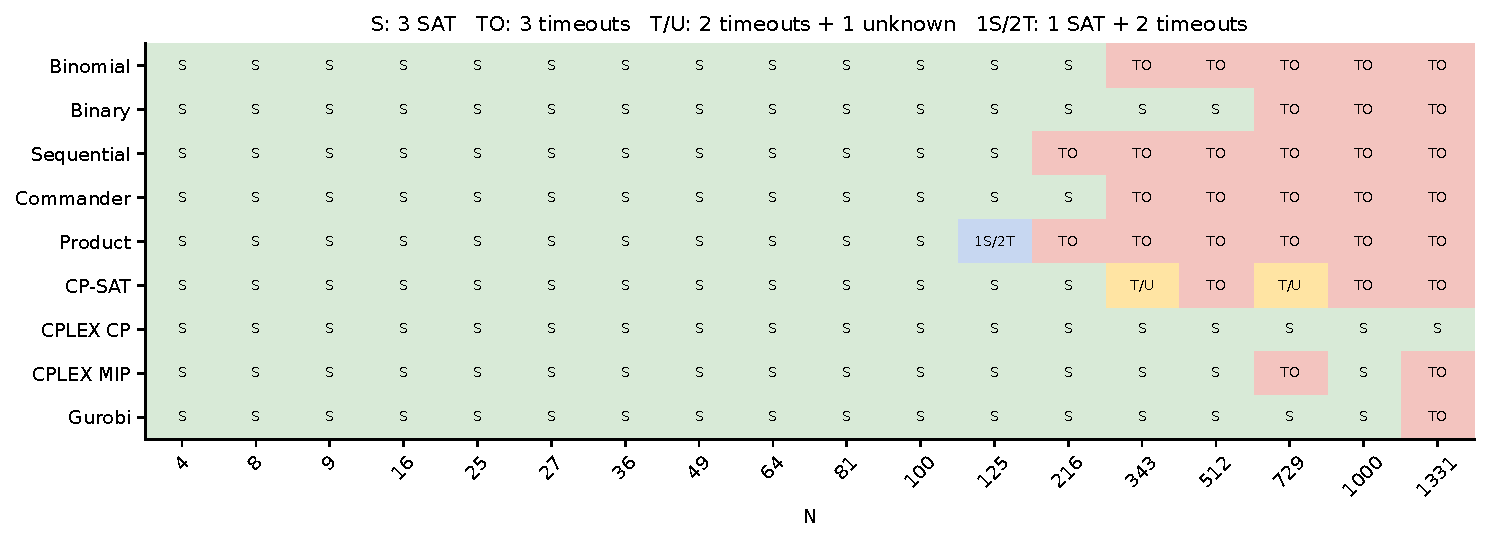
\includegraphics[width=\linewidth]{figures/status_matrix.pdf}
\caption{Trạng thái trên 18 kích thước. S: ba lượt SAT; TO: ba TIMEOUT; T/U: hai TIMEOUT và một UNKNOWN; 1S/2T: một SAT và hai TIMEOUT.}
\label{fig:status}
\end{figure}
CPLEX CP hoàn tất cả 18 kích thước; Gurobi hoàn tất 17; CPLEX MIP 16; Binary 15; Binomial, Commander và CP-SAT cùng 13; Sequential 12; Product hoàn tất đủ ba lượt ở 11 kích thước và có một lượt thành công thêm tại $N=125$. Tất cả cấu hình đều đã được thử ở mọi kích thước, nên không còn sự nhập nhằng giữa bỏ qua trước chạy và timeout trong đánh giá mức độ hoàn tất.

\begin{figure}[pos=H]\centering
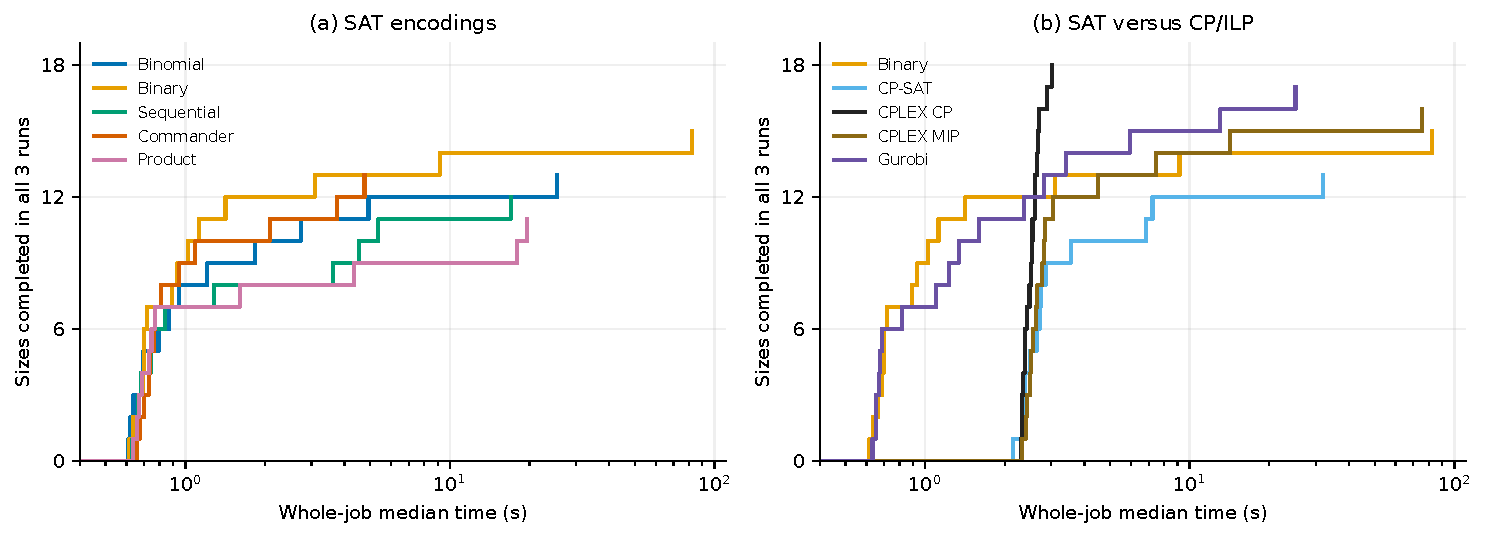
\includegraphics[width=\linewidth]{figures/cactus.pdf}
\caption{Số kích thước hoàn tất đủ 3/3 theo ngưỡng trung vị total. Chỉ các nhóm hoàn tất được tính; đường kết thúc ở số kích thước đã giải, không thay lượt chưa hoàn tất bằng điểm 100 giây.}
\label{fig:cactus}
\end{figure}

\subsection{So sánh số biến và số mệnh đề}
\begin{table}[pos=H]
\centering
\footnotesize
\caption{Số biến CNF đầy đủ của năm mã hóa.}
\label{tab:variables}
\setlength{\tabcolsep}{4pt}
\begin{tabular}{@{}lrrrrr@{}}
\toprule
$N$ & Binomial & Binary & Sequential & Commander & Product \\
\midrule
4 & 16 & 48 & 46 & 36 & 16 \\
8 & 64 & 174 & 262 & 154 & 236 \\
9 & 81 & 229 & 341 & 189 & 289 \\
16 & 256 & 572 & 1\,174 & 744 & 820 \\
25 & 625 & 1\,241 & 2\,965 & 1\,813 & 2\,533 \\
27 & 729 & 1\,405 & 3\,473 & 2\,061 & 2\,937 \\
36 & 1\,296 & 2\,328 & 6\,254 & 3\,876 & 4\,732 \\
49 & 2\,401 & 3\,901 & 11\,701 & 7\,265 & 8\,097 \\
64 & 4\,096 & 6\,136 & 20\,086 & 12\,442 & 12\,476 \\
81 & 6\,561 & 9\,441 & 32\,309 & 19\,449 & 18\,221 \\
100 & 10\,000 & 13\,678 & 49\,390 & 30\,536 & 26\,104 \\
125 & 15\,625 & 20\,353 & 77\,365 & 47\,257 & 37\,749 \\
216 & 46\,656 & 55\,988 & 231\,974 & 140\,030 & 94\,672 \\
343 & 117\,649 & 134\,109 & 586\,177 & 355\,969 & 220\,149 \\
512 & 262\,144 & 287\,730 & 1\,307\,638 & 789\,618 & 459\,472 \\
729 & 531\,441 & 571\,069 & 2\,652\,821 & 1\,595\,061 & 859\,721 \\
1000 & 1\,000\,000 & 1\,055\,888 & 4\,993\,990 & 3\,013\,684 & 1\,514\,732 \\
1331 & 1\,771\,561 & 1\,851\,197 & 8\,849\,809 & 5\,326\,901 & 2\,536\,565 \\
\bottomrule
\end{tabular}
\par\smallskip\begin{minipage}{\linewidth}\footnotesize Commander và Product đều là bản đệ quy. Số đếm theo công thức trước tiền xử lý; TIMEOUT không làm giảm kích thước mô hình đầy đủ. Không bao gồm clause học.\end{minipage}
\end{table}

\begin{table}[pos=H]
\centering
\footnotesize
\caption{Số clause đầu vào của năm mã hóa.}
\label{tab:clauses}
\setlength{\tabcolsep}{4pt}
\begin{tabular}{@{}lrrrrr@{}}
\toprule
$N$ & Binomial & Binary & Sequential & Commander & Product \\
\midrule
4 & 84 & 120 & 104 & 124 & 84 \\
8 & 744 & 728 & 592 & 634 & 652 \\
9 & 1\,074 & 1\,114 & 774 & 822 & 826 \\
16 & 6\,352 & 3\,928 & 2\,720 & 3\,176 & 2\,804 \\
25 & 24\,850 & 11\,806 & 6\,950 & 8\,018 & 7\,638 \\
27 & 31\,410 & 13\,890 & 8\,154 & 9\,294 & 8\,930 \\
36 & 75\,252 & 28\,320 & 14\,760 & 17\,276 & 15\,292 \\
49 & 191\,394 & 54\,866 & 27\,734 & 32\,526 & 27\,742 \\
64 & 428\,864 & 95\,576 & 47\,744 & 55\,990 & 45\,620 \\
81 & 872\,802 & 172\,694 & 76\,950 & 89\,322 & 70\,710 \\
100 & 1\,646\,900 & 269\,024 & 117\,800 & 138\,628 & 106\,292 \\
125 & 3\,224\,250 & 426\,574 & 184\,750 & 216\,062 & 161\,882 \\
216 & 16\,703\,352 & 1\,449\,224 & 555\,120 & 647\,438 & 458\,024 \\
343 & 67\,021\,514 & 4\,060\,266 & 1\,404\,242 & 1\,644\,150 & 1\,121\,094 \\
512 & 223\,173\,120 & 9\,262\,424 & 3\,134\,464 & 3\,662\,390 & 2\,439\,384 \\
729 & 644\,639\,634 & 20\,558\,002 & 6\,361\,254 & 7\,421\,982 & 4\,824\,850 \\
1000 & 1\,664\,669\,000 & 39\,300\,904 & 11\,978\,000 & 13\,999\,546 & 8\,907\,744 \\
1331 & 3\,926\,372\,802 & 75\,151\,050 & 21\,229\,450 & 24\,787\,642 & 15\,533\,774 \\
\bottomrule
\end{tabular}
\par\smallskip\begin{minipage}{\linewidth}\footnotesize Commander và Product đều là bản đệ quy. Số đếm theo công thức trước tiền xử lý; TIMEOUT không làm giảm kích thước mô hình đầy đủ. Không bao gồm clause học.\end{minipage}
\end{table}

\begin{figure}[pos=H]\centering
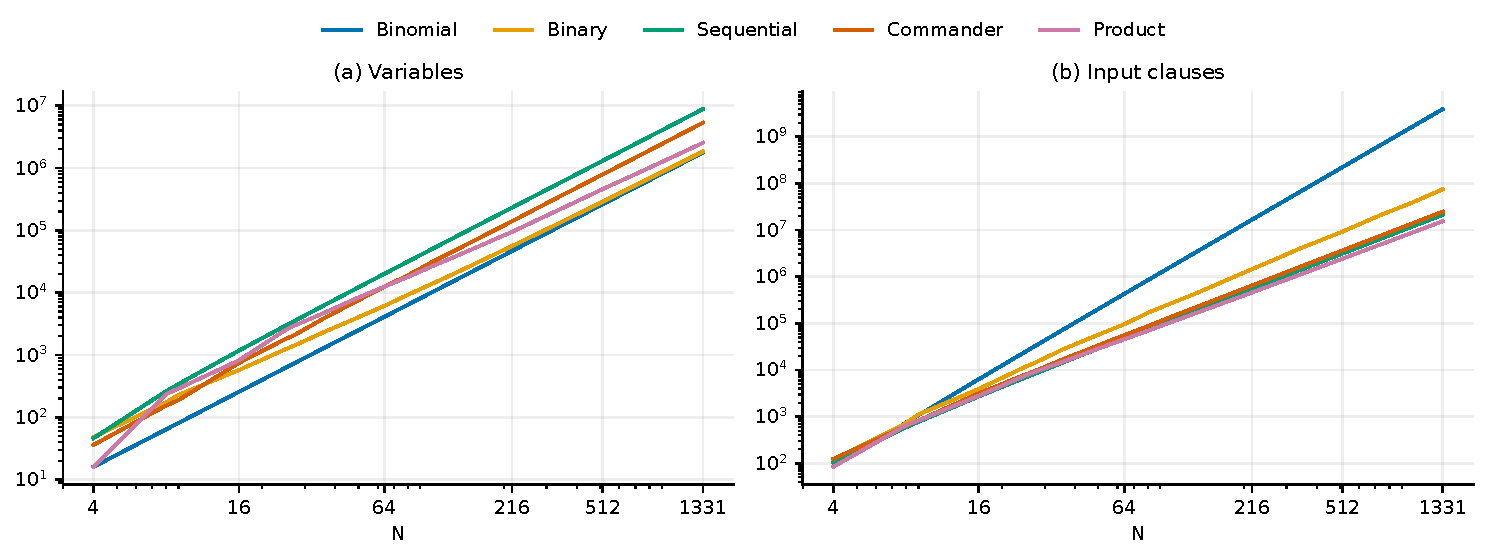
\includegraphics[width=\linewidth]{figures/formula_sizes.pdf}
\caption{Kích thước CNF đầy đủ theo công thức. Hai trục dùng thang log. Commander/Product là bản đệ quy; điểm có số đếm không chứng minh lượt tương ứng đã sinh hoặc nạp hết CNF.}
\label{fig:counts}
\end{figure}
Binomial không thêm biến phụ nên có ít biến nhất, nhưng số clause tăng nhanh nhất. Tại $N=1331$, Binomial có 1\,771\,561 biến và 3\,926\,372\,802 clause. Binary chỉ tăng lên 1\,851\,197 biến, nhưng vẫn có 75\,151\,050 clause. Sequential có 8\,849\,809 biến và 21\,229\,450 clause; Commander có 5\,326\,901 biến và 24\,787\,642 clause; Product có 2\,536\,565 biến và 15\,533\,774 clause.

Như vậy Product có ít clause nhất tại kích thước lớn nhất, còn Sequential dùng nhiều biến nhất trong năm cấu hình. Các con số phù hợp với cấu trúc: Binary chia sẻ một mã bit trong mỗi nhóm, Sequential cần chuỗi gần bằng độ dài nhóm, Commander tạo các tầng đại diện và Product phân rã qua các tập tọa độ. Tuy nhiên, các đặc trưng kích thước chưa đủ dự đoán khả năng hoàn tất trong 100 giây, như các kết quả thời gian sau đây cho thấy.

\subsection{So sánh thời gian giữa các mã hóa SAT}
\begin{table}[pos=H]
\centering
\small
\caption{Thời gian sinh, nạp và giải SAT: $T_{\mathrm{work}}$ (giây).}
\label{tab:sat_work}
\setlength{\tabcolsep}{4pt}
\begin{tabular}{@{}lrrrrr@{}}
\toprule
$N$ & Binomial & Binary & Sequential & Commander & Product \\
\midrule
4 & 0.000295 & 0.000424 & 0.000388 & 0.000500 & 0.000322 \\
8 & 0.001347 & 0.001974 & 0.001213 & 0.001939 & 0.002030 \\
9 & 0.001568 & 0.002136 & 0.001609 & 0.002271 & 0.002592 \\
16 & 0.0306 & 0.0183 & 0.0166 & 0.0779 & 0.0143 \\
25 & 0.0335 & 0.0307 & 0.0528 & 0.0366 & 0.0353 \\
27 & 0.0516 & 0.0275 & 0.1031 & 0.0642 & 0.1004 \\
36 & 0.0953 & 0.0933 & 0.1389 & 0.1180 & 0.0999 \\
49 & 0.2141 & 0.2645 & 0.6036 & 0.1184 & 0.7945 \\
64 & 0.5004 & 0.2273 & 3.902 & 0.3088 & 18.958 \\
81 & 1.091 & 0.3448 & 2.945 & 0.3738 & 3.648 \\
100 & 1.894 & 0.4430 & 4.715 & 1.395 & 17.319 \\
125 & 3.944 & 0.7298 & 16.299 & 3.015 & 1S+2TO \\
216 & 22.912 & 2.296 & TO & 3.940 & TO \\
343 & TO & 8.089 & TO & TO & TO \\
512 & TO & 81.088 & TO & TO & TO \\
729 & TO & TO & TO & TO & TO \\
1000 & TO & TO & TO & TO & TO \\
1331 & TO & TO & TO & TO & TO \\
\bottomrule
\end{tabular}
\par\smallskip\begin{minipage}{\linewidth}\footnotesize Giá trị số: trung vị của ba lượt SAT có nghiệm hợp lệ. TO: ba TIMEOUT; 2TO+1U: hai TIMEOUT và một UNKNOWN; 1S+2TO: một SAT và hai TIMEOUT. Không thay lượt chưa hoàn tất bằng 0 hoặc 100 giây.\end{minipage}
\end{table}

\begin{table}[pos=H]
\centering
\small
\caption{Thời gian toàn lượt SAT: $T_{\mathrm{total}}$ (giây).}
\label{tab:sat_total}
\setlength{\tabcolsep}{4pt}
\begin{tabular}{@{}lrrrrr@{}}
\toprule
$N$ & Binomial & Binary & Sequential & Commander & Product \\
\midrule
4 & 0.6085 & 0.6645 & 0.6297 & 0.7000 & 0.6335 \\
8 & 0.6199 & 0.6987 & 0.6622 & 0.6723 & 0.6663 \\
9 & 0.6376 & 0.6152 & 0.6808 & 0.6593 & 0.6569 \\
16 & 0.7921 & 0.6893 & 0.6653 & 0.7351 & 0.6843 \\
25 & 0.6953 & 0.6344 & 0.7505 & 0.7693 & 0.7283 \\
27 & 0.6795 & 0.6968 & 0.7408 & 0.7276 & 0.7457 \\
36 & 0.9440 & 0.7163 & 0.8390 & 0.7624 & 0.7660 \\
49 & 0.8694 & 0.9330 & 1.282 & 0.8098 & 1.607 \\
64 & 1.212 & 0.8928 & 4.530 & 0.9501 & 19.578 \\
81 & 1.838 & 1.024 & 3.614 & 1.092 & 4.347 \\
100 & 2.731 & 1.123 & 5.370 & 2.084 & 17.965 \\
125 & 4.929 & 1.419 & 16.970 & 3.745 & 1S+2TO \\
216 & 25.469 & 3.085 & TO & 4.760 & TO \\
343 & TO & 9.145 & TO & TO & TO \\
512 & TO & 82.550 & TO & TO & TO \\
729 & TO & TO & TO & TO & TO \\
1000 & TO & TO & TO & TO & TO \\
1331 & TO & TO & TO & TO & TO \\
\bottomrule
\end{tabular}
\par\smallskip\begin{minipage}{\linewidth}\footnotesize Giá trị số: trung vị của ba lượt SAT có nghiệm hợp lệ. TO: ba TIMEOUT; 2TO+1U: hai TIMEOUT và một UNKNOWN; 1S+2TO: một SAT và hai TIMEOUT. Không thay lượt chưa hoàn tất bằng 0 hoặc 100 giây.\end{minipage}
\end{table}

\begin{figure}[pos=H]\centering
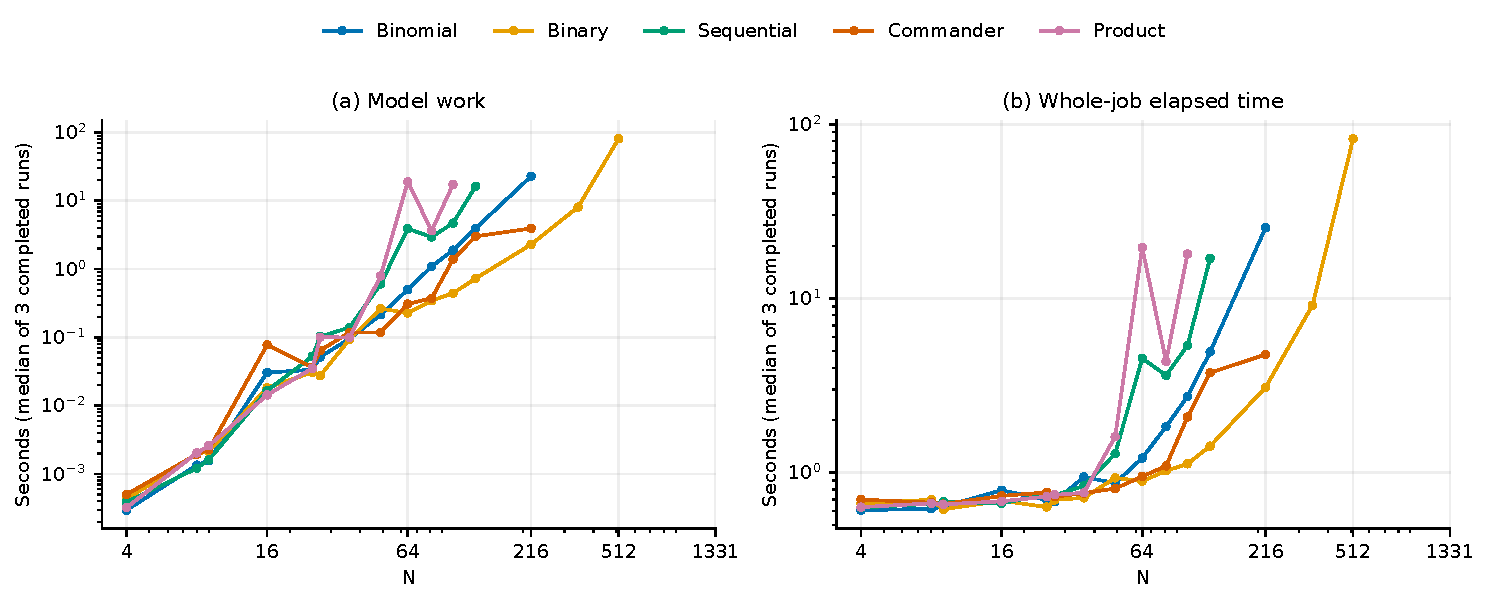
\includegraphics[width=\linewidth]{figures/sat_runtime.pdf}
\caption{Trung vị thời gian SAT: phần xử lý mô hình và giải (trái), toàn lượt (phải). Chỉ vẽ các nhóm hoàn tất 3/3; các trục thời gian dùng thang log.}
\label{fig:sat-time}
\end{figure}
Binary đạt mức độ hoàn tất cao nhất trong các cấu hình SAT: 15/18 kích thước, đến $N=512$. Tại $N=216$, trung vị work của Binary là 2.296 giây, Commander 3.940 giây và Binomial 22.912 giây; Sequential và Product đều timeout. Tại $N=512$, Binary cần 81.088 giây work và 82.550 giây total, còn bốn mã hóa SAT khác đều timeout. Đây là ưu thế của Binary trong bộ cài đặt, backend và tập đầu vào hiện tại, không phải một thứ tự ưu việt cho mọi bài SAT.

Ở kích thước nhỏ, thứ hạng thay đổi: Binomial nhanh nhất theo work tại $N=4,9$, Sequential tại $N=8$ và Product tại $N=16$. Tốc độ cũng không tăng đơn điệu theo $N$: work của Product giảm từ 18.958 giây tại $N=64$ xuống 3.648 giây tại $N=81$, dù công thức lớn hơn. Vì thế không nên suy thời gian ở $N$ tiếp theo chỉ từ đường tăng số clause.

\begin{table}[pos=H]
\centering
\small
\caption{Đối chiếu với Binomial trên tập cả hai hoàn tất 3/3.}
\label{tab:pairwise_binomial}
\setlength{\tabcolsep}{4pt}
\begin{tabular}{@{}lrrrr@{}}
\toprule
Encoding & $|S|$ & Nhanh hơn & Chậm hơn & Hệ số hình học \\
\midrule
Binary & 13 & 9 & 4 & 1.762 \\
Sequential & 12 & 2 & 10 & 0.534 \\
Commander & 13 & 6 & 7 & 1.145 \\
Product & 11 & 1 & 10 & 0.426 \\
\bottomrule
\end{tabular}
\par\smallskip\begin{minipage}{\linewidth}\footnotesize Dùng $T_{work}$. Hệ số lớn hơn 1 nghĩa là nhanh hơn Binomial. Tập so sánh khác nhau giữa các hàng, nên không dùng làm xếp hạng chung.\end{minipage}
\end{table}

Với $S$ là tập kích thước cả một mã hóa $E$ và Binomial đều hoàn tất đủ ba lượt, hệ số đối chiếu được tính bằng
\[
G_E=\exp\left(\frac{1}{|S|}\sum_{N\in S}
\log\frac{\widetilde T_{\mathrm{work}}^{\mathrm{Binomial}}(N)}
{\widetilde T_{\mathrm{work}}^{E}(N)}\right).
\]
Binary nhanh hơn Binomial ở 9/13 kích thước chung, hệ số hình học 1.762. Commander nhanh hơn ở 6/13, hệ số 1.145. Sequential và Product có hệ số lần lượt 0.534 và 0.426 trên các tập chung riêng. Những hệ số này không tính các lượt chưa hoàn tất và tập $S$ khác nhau, nên cần đọc cùng bảng mức độ hoàn tất, không dùng riêng để xếp hạng toàn bộ phương pháp.

\begin{figure}[pos=H]\centering
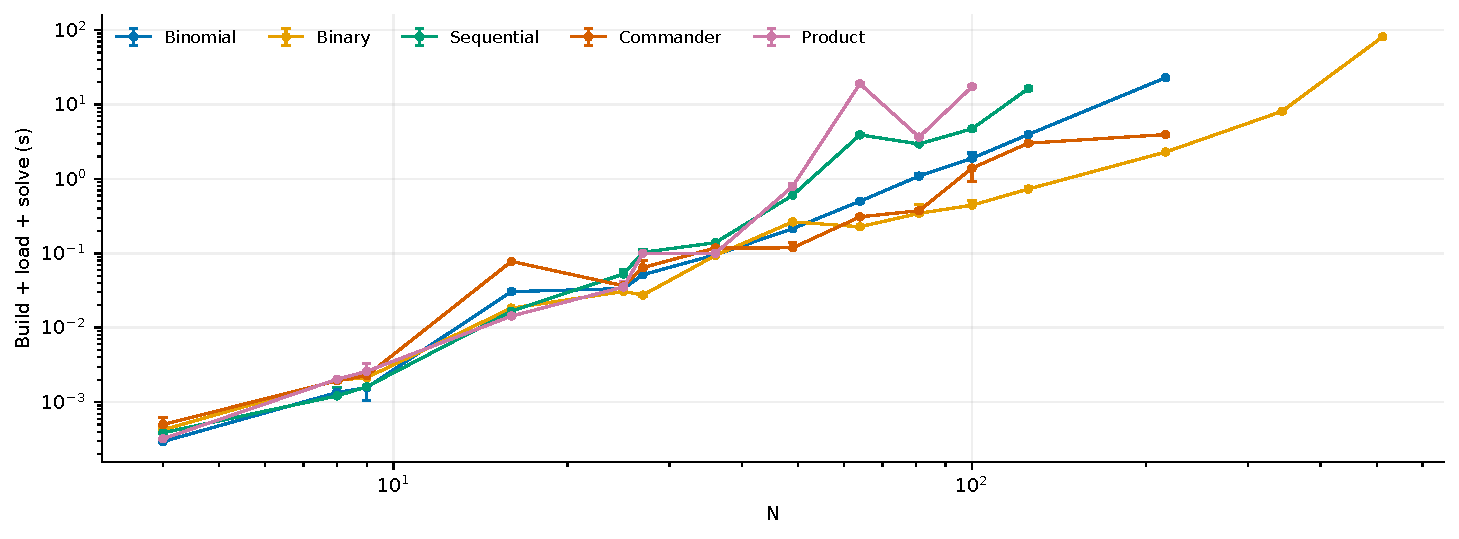
\includegraphics[width=\linewidth]{figures/sat_iqr.pdf}
\caption{Trung vị và khoảng từ Q1 đến Q3 của work trên ba lần lặp hoàn tất. Thanh sai số mô tả độ phân tán, không phải khoảng tin cậy.}
\label{fig:iqr}
\end{figure}
Ví dụ Binary tại $N=81$ có IQR/work trung vị 35.9\%, trong khi tại $N=216$ là 3.0\%. Khác biệt này cho thấy cần giữ các lượt thô thay vì chỉ lưu một thời gian duy nhất. Ba lần lặp chưa đủ để đưa ra kiểm định thống kê mạnh hoặc suy diễn độ ổn định trên nhiều máy.

\subsection{Vì sao ít clause hơn chưa chắc giải nhanh hơn?}
\begin{table}[pos=H]
\centering
\small
\caption{Số clause và công việc tìm kiếm của Glucose3 tại N=64.}
\label{tab:counterexample}
\setlength{\tabcolsep}{4pt}
\begin{tabular}{@{}lrrrr@{}}
\toprule
Mã hóa & Clause & Solve (s) & Xung đột & Lan truyền \\
\midrule
Binomial & 428\,864 & 0.0229 & 317 & 30\,574 \\
Binary & 95\,576 & 0.1026 & 876 & 220\,738 \\
Sequential & 47\,744 & 3.839 & 9\,471 & 3\,899\,877 \\
Commander & 55\,990 & 0.2145 & 1\,231 & 486\,461 \\
Product & 45\,620 & 18.884 & 45\,055 & 12\,682\,652 \\
\bottomrule
\end{tabular}
\par\smallskip\begin{minipage}{\linewidth}\footnotesize Bộ đếm xung đột và lan truyền trùng nhau giữa ba lượt của mỗi mã hóa ở N=64. Thời gian là trung vị; các mã hóa có cấu trúc khác nhau.\end{minipage}
\end{table}

Tại $N=64$, Product chỉ có 45\,620 clause nhưng solve trung vị khoảng 18.884 giây. Binomial có 428\,864 clause, nhiều hơn khoảng 9.4 lần, nhưng solve chỉ khoảng 0.0229 giây. Product ghi nhận 45\,055 xung đột và 12\,682\,652 lần lan truyền, trong khi Binomial lần lượt là 317 và 30\,574. Sequential cũng có ít clause hơn Binary nhưng thời gian solve lớn hơn.

Các số đếm tìm kiếm hỗ trợ nhận xét rằng sự khác biệt không chỉ nằm ở chi phí Python: cấu trúc ràng buộc dẫn tới lượng công việc khác nhau bên trong Glucose3. Chúng chưa chứng minh duy nhất một cơ chế gây chậm, vì thứ tự clause, đánh số biến, quyết định phân nhánh và clause học đều có thể ảnh hưởng. Kết luận phù hợp là kích thước CNF cần được đánh giá cùng hành vi tìm kiếm thực tế.

Tại điểm này, bộ đếm xung đột và lan truyền trùng nhau giữa ba lần lặp của mỗi mã hóa. Do đó không có cơ sở quy mọi dao động thời gian cho sự ngẫu nhiên của SAT solver. Các lượt lặp với cấu hình seed không đổi còn phản ánh biến động của môi trường thực thi.

\subsection{Chi phí khởi động và phân rã thời gian}
\begin{table}[pos=H]
\centering
\small
\caption{Thành phần thời gian SAT tại N=4 (mili giây).}
\label{tab:small_n}
\setlength{\tabcolsep}{4pt}
\begin{tabular}{@{}lrrrrr@{}}
\toprule
Mã hóa & Khởi động & Thiết lập & $T_{work}$ & Solve & $T_{total}$ \\
\midrule
Binomial & 478.149 & 106.422 & 0.295 & 0.061 & 608.488 \\
Binary & 513.512 & 131.196 & 0.424 & 0.085 & 664.473 \\
Sequential & 504.904 & 112.106 & 0.388 & 0.064 & 629.726 \\
Commander & 547.531 & 125.069 & 0.500 & 0.079 & 700.005 \\
Product & 488.594 & 118.623 & 0.322 & 0.063 & 633.508 \\
\bottomrule
\end{tabular}
\par\smallskip\begin{minipage}{\linewidth}\footnotesize Mỗi cột là một trung vị riêng. Trung vị tổng không nhất thiết bằng tổng các trung vị thành phần.\end{minipage}
\end{table}

Ở $N=4$, work của các mã hóa SAT nằm khoảng 0.295--0.500 mili giây, trong khi total khoảng 608--700 mili giây. Phần khởi động và thiết lập chiếm phần lớn khoảng chênh lệch. So total của chương trình có worker riêng với solve của chương trình chạy sẵn trong một tiến trình sẽ tạo khác biệt hàng nghìn lần dù công việc SAT gần tương đương.

\begin{table}[pos=H]
\centering
\small
\caption{Phân rã thời gian tại N=216 (giây).}
\label{tab:phase_216}
\setlength{\tabcolsep}{4pt}
\begin{tabular}{@{}lrrrrr@{}}
\toprule
Phương pháp & Build & Load & Solve & $T_{work}$ & $T_{total}$ \\
\midrule
Binomial & 5.943 & 15.416 & 1.237 & 22.912 & 25.469 \\
Binary & 0.5317 & 1.298 & 0.4549 & 2.296 & 3.085 \\
Sequential & TO & TO & TO & TO & TO \\
Commander & 0.3939 & 0.7232 & 2.818 & 3.940 & 4.760 \\
Product & TO & TO & TO & TO & TO \\
CP-SAT & 0.006869 & -- & 29.904 & 29.911 & 32.014 \\
CPLEX CP & 0.003330 & -- & 0.0830 & 0.0863 & 2.422 \\
CPLEX MIP & 0.6064 & -- & 1.150 & 1.768 & 4.501 \\
Gurobi & 0.7344 & -- & 1.936 & 2.673 & 3.397 \\
\bottomrule
\end{tabular}
\par\smallskip\begin{minipage}{\linewidth}\footnotesize Mỗi cột là một trung vị riêng; tổng các trung vị pha có thể khác trung vị work. Load chỉ áp dụng cho SAT; dấu -- của native không phải một pha nạp được đo bằng 0.\end{minipage}
\end{table}

Tại $N=216$, Binomial có trung vị build 5.943 giây và load 15.416 giây, lớn hơn rõ rệt solve 1.237 giây. Binary giảm phần build/load xuống 0.532 và 1.298 giây; Commander có build/load thấp hơn nữa nhưng solve 2.818 giây, lớn hơn Binary 0.455 giây. Các trung vị pha không bắt buộc cộng lại bằng trung vị work, vì chúng có thể đến từ các lượt khác nhau.

\begin{figure}[pos=H]\centering
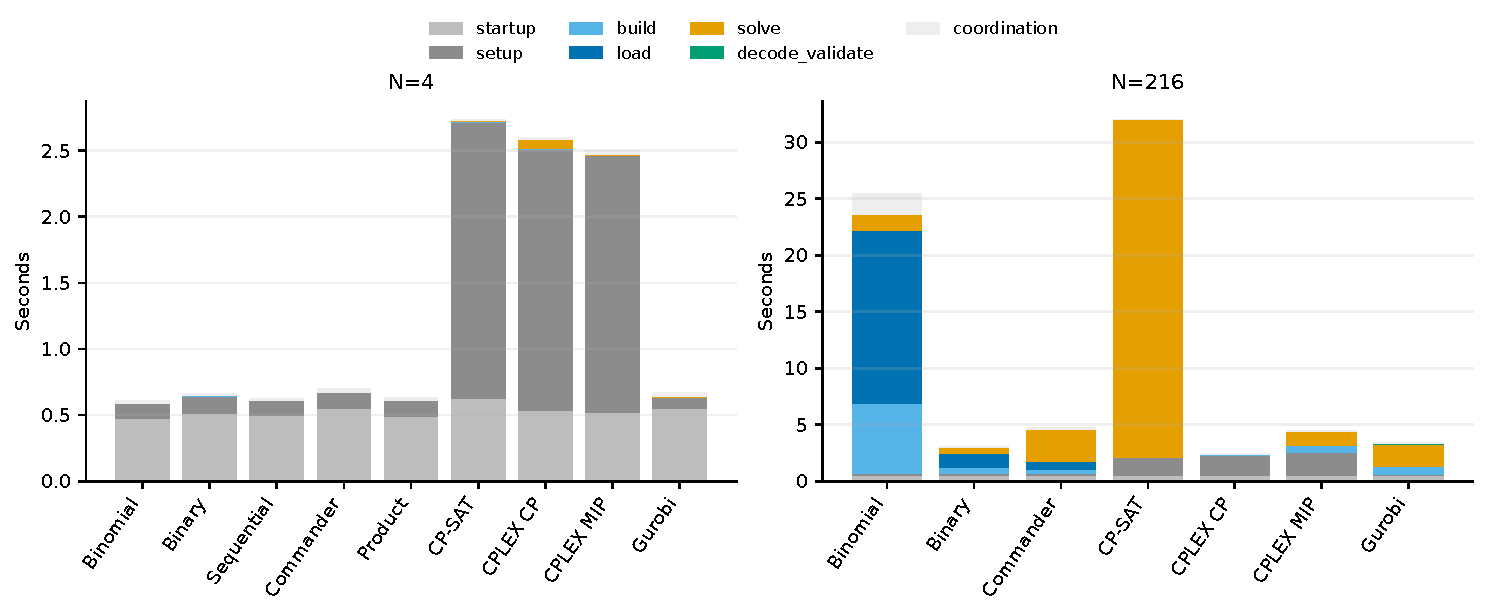
\includegraphics[width=\linewidth]{figures/phase_breakdown.pdf}
\caption{Phân rã một lượt thực tại $N=4$ và $N=216$. Với mỗi cấu hình, chọn lượt có total ở vị trí trung vị; các cột chồng vì vậy thuộc cùng một lượt. Coordination là phần total còn lại sau các pha được ghi.}
\label{fig:phases}
\end{figure}

\subsection{Đối sánh SAT với CP-SAT, CPLEX CP, CPLEX MIP và Gurobi}
\begin{table}[pos=H]
\centering
\small
\caption{Thời gian xây mô hình và gọi giải CP/ILP: $T_{\mathrm{work}}$ (giây).}
\label{tab:native_work}
\setlength{\tabcolsep}{4pt}
\begin{tabular}{@{}lrrrr@{}}
\toprule
$N$ & CP-SAT & CPLEX CP & CPLEX MIP & Gurobi \\
\midrule
4 & 0.0142 & 0.0694 & 0.0146 & 0.0106 \\
8 & 0.0217 & 0.0642 & 0.0125 & 0.009471 \\
9 & 0.0237 & 0.0617 & 0.0138 & 0.009109 \\
16 & 0.0459 & 0.0569 & 0.0214 & 0.0393 \\
25 & 0.0962 & 0.0655 & 0.0340 & 0.0202 \\
27 & 0.1112 & 0.0609 & 0.0350 & 0.0201 \\
36 & 0.2155 & 0.0621 & 0.0528 & 0.0311 \\
49 & 0.4258 & 0.0619 & 0.0833 & 0.1921 \\
64 & 0.7318 & 0.0714 & 0.1399 & 0.0758 \\
81 & 1.395 & 0.0738 & 0.1896 & 0.3590 \\
100 & 3.372 & 0.0727 & 0.2943 & 0.4322 \\
125 & 4.959 & 0.0734 & 0.4708 & 1.187 \\
216 & 29.911 & 0.0863 & 1.768 & 2.673 \\
343 & 2TO+1U & 0.1040 & 4.965 & 1.969 \\
512 & TO & 0.1832 & 10.909 & 4.719 \\
729 & 2TO+1U & 0.2148 & TO & 10.777 \\
1000 & TO & 0.4710 & 72.076 & 21.868 \\
1331 & TO & 0.5211 & TO & TO \\
\bottomrule
\end{tabular}
\par\smallskip\begin{minipage}{\linewidth}\footnotesize Giá trị số: trung vị của ba lượt SAT có nghiệm hợp lệ. TO: ba TIMEOUT; 2TO+1U: hai TIMEOUT và một UNKNOWN; 1S+2TO: một SAT và hai TIMEOUT. Không thay lượt chưa hoàn tất bằng 0 hoặc 100 giây.\end{minipage}
\end{table}

\begin{table}[pos=H]
\centering
\small
\caption{Thời gian toàn lượt CP/ILP (giây).}
\label{tab:native_total}
\setlength{\tabcolsep}{4pt}
\begin{tabular}{@{}lrrrr@{}}
\toprule
$N$ & CP-SAT & CPLEX CP & CPLEX MIP & Gurobi \\
\midrule
4 & 2.735 & 2.598 & 2.499 & 0.6738 \\
8 & 2.338 & 2.545 & 2.324 & 0.6705 \\
9 & 2.486 & 2.352 & 2.775 & 0.6508 \\
16 & 2.145 & 2.295 & 2.626 & 0.8176 \\
25 & 2.358 & 2.522 & 2.505 & 0.6522 \\
27 & 2.382 & 2.480 & 2.397 & 0.6327 \\
36 & 2.638 & 2.376 & 2.832 & 0.6870 \\
49 & 2.713 & 2.314 & 2.423 & 1.338 \\
64 & 2.851 & 2.319 & 2.652 & 1.231 \\
81 & 3.547 & 2.697 & 2.555 & 1.597 \\
100 & 6.843 & 2.653 & 2.812 & 1.099 \\
125 & 7.232 & 2.380 & 3.042 & 2.363 \\
216 & 32.014 & 2.422 & 4.501 & 3.397 \\
343 & 2TO+1U & 2.526 & 7.466 & 2.814 \\
512 & TO & 2.597 & 14.195 & 5.927 \\
729 & 2TO+1U & 2.665 & TO & 13.066 \\
1000 & TO & 2.888 & 75.464 & 25.111 \\
1331 & TO & 3.010 & TO & TO \\
\bottomrule
\end{tabular}
\par\smallskip\begin{minipage}{\linewidth}\footnotesize Giá trị số: trung vị của ba lượt SAT có nghiệm hợp lệ. TO: ba TIMEOUT; 2TO+1U: hai TIMEOUT và một UNKNOWN; 1S+2TO: một SAT và hai TIMEOUT. Không thay lượt chưa hoàn tất bằng 0 hoặc 100 giây.\end{minipage}
\end{table}

\begin{figure}[pos=H]\centering
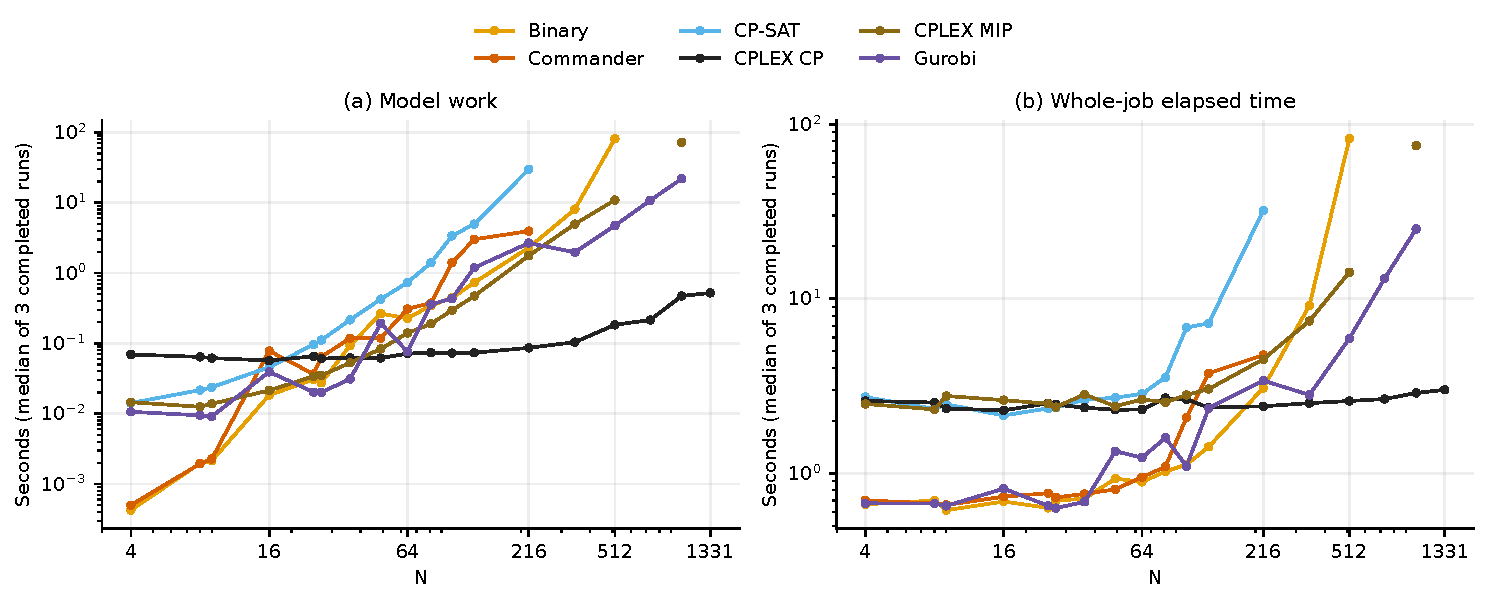
\includegraphics[width=\linewidth]{figures/native_runtime.pdf}
\caption{Binary, Commander và bốn phương pháp đối sánh. Hình tách work với total; chỉ gồm nhóm hoàn tất 3/3.}
\label{fig:native-time}
\end{figure}
CPLEX CP đạt độ bao phủ lớn nhất và có work thấp ở các kích thước lớn: 0.0863 giây tại $N=216$, 0.1832 giây tại $N=512$ và 0.5211 giây tại $N=1331$. Total tương ứng khoảng 2.422, 2.597 và 3.010 giây. Sự chênh lệch work--total phản ánh phần thiết lập còn đáng kể ngay cả khi lời gọi CP hoàn thành nhanh.

Ở $N=512$, Binary cần 81.088 giây work, CPLEX MIP 10.909 giây và Gurobi 4.719 giây. Tại $N=1000$, CPLEX MIP hoàn tất với work 72.076 giây và Gurobi với 21.868 giây, trong khi mọi SAT encoding đều timeout. CPLEX MIP timeout ở $N=729$ nhưng hoàn tất ở $N=1000$; điều này tiếp tục cho thấy độ khó tìm kiếm không đơn điệu theo kích thước. CP-SAT hoàn tất đến $N=216$, rồi các kích thước lớn hơn kết thúc bằng TIMEOUT hoặc UNKNOWN.

\begin{table}[pos=H]
\centering
\small
\caption{Số kích thước có trung vị nhanh nhất trên tập chung.}
\label{tab:matched_winners}
\setlength{\tabcolsep}{4pt}
\begin{tabular}{@{}lrr@{}}
\toprule
Phương pháp & Theo $T_{work}$ & Theo $T_{total}$ \\
\midrule
Binomial & 2 & 2 \\
Binary & 0 & 4 \\
Sequential & 1 & 1 \\
Commander & 0 & 1 \\
Product & 1 & 0 \\
CP-SAT & 0 & 0 \\
CPLEX CP & 4 & 0 \\
CPLEX MIP & 0 & 0 \\
Gurobi & 3 & 3 \\
\bottomrule
\end{tabular}
\par\smallskip\begin{minipage}{\linewidth}\footnotesize Tập chung gồm 11 kích thước: 4, 8, 9, 16, 25, 27, 36, 49, 64, 81, 100. Mỗi kích thước có trọng số bằng nhau; không thay thế đánh giá mức độ hoàn tất.\end{minipage}
\end{table}

Tập mà cả chín cấu hình đều hoàn tất gồm 11 kích thước từ 4 đến 100 trong $\mathcal N$. Theo work, CPLEX CP nhanh nhất ở bốn kích thước, Gurobi ở ba, Binomial ở hai, Sequential và Product mỗi phương pháp ở một. Theo total, Binary dẫn đầu ở bốn kích thước còn CPLEX CP không dẫn đầu ở kích thước nào trong tập chung này. Hai cách đo trả lời hai câu hỏi khác nhau: tốc độ xử lý mô hình và giải sau thiết lập, hoặc độ trễ thực thi toàn lượt.

\begin{table}[pos=H]
\centering
\small
\caption{Kích thước mô hình CP và MIP ở giao diện người dùng.}
\label{tab:native_size}
\setlength{\tabcolsep}{4pt}
\begin{tabular}{@{}lrrrr@{}}
\toprule
$N$ & Biến CP & AllDifferent & Biến MIP & Ràng buộc MIP \\
\midrule
4 & 4 & 3 & 16 & 22 \\
216 & 216 & 3 & 46\,656 & 1\,294 \\
1331 & 1331 & 3 & 1\,771\,561 & 7\,984 \\
\bottomrule
\end{tabular}
\par\smallskip\begin{minipage}{\linewidth}\footnotesize Không quy đổi biến nguyên hoặc ràng buộc mức cao thành biến/clause CNF. Không phải số lượng bên trong solver sau presolve.\end{minipage}
\end{table}

Ba AllDifferent có thể biểu diễn các quan hệ rộng trên miền của $N$ biến nguyên, trong khi mô hình ô cờ SAT/MIP sử dụng $N^2$ biến Boolean/nhị phân. Đây là khác biệt về cách biểu diễn mà backend nhận được, không phải bằng chứng rằng ba ràng buộc CP chỉ có chi phí bằng ba clause. Thực nghiệm so sánh cả mô hình lẫn bộ giải; không cô lập riêng chất lượng thuật toán nội bộ của các engine.

\subsection{RSS và tài nguyên bộ nhớ}
\begin{table}[pos=H]
\centering
\small
\caption{Trung vị đỉnh RSS quan sát (SAT, MiB).}
\label{tab:sat_ram}
\setlength{\tabcolsep}{4pt}
\begin{tabular}{@{}lrrrrr@{}}
\toprule
$N$ & Binomial & Binary & Sequential & Commander & Product \\
\midrule
4 & 27.8 & 27.8 & 27.8 & 27.8 & 27.9 \\
8 & 27.6 & 27.8 & 27.8 & 27.7 & 27.9 \\
9 & 28.1 & 28.2 & 27.9 & 28.0 & 27.8 \\
16 & 29.2 & 28.5 & 28.2 & 28.9 & 28.2 \\
25 & 29.4 & 28.4 & 29.8 & 29.8 & 29.6 \\
27 & 31.2 & 28.7 & 30.0 & 29.9 & 30.1 \\
36 & 33.2 & 30.4 & 31.6 & 31.3 & 30.6 \\
49 & 39.8 & 34.2 & 34.5 & 32.6 & 36.8 \\
64 & 52.4 & 36.0 & 44.5 & 36.8 & 61.2 \\
81 & 71.9 & 40.7 & 45.8 & 39.9 & 49.2 \\
100 & 119.9 & 46.0 & 52.3 & 47.9 & 67.1 \\
125 & 184.2 & 55.6 & 74.0 & 59.5 & 154.8$^{\dagger}$ \\
216 & 1120.7 & 105.4 & 325.0$^{\dagger}$ & 104.2 & 206.9$^{\dagger}$ \\
343 & 3032.1$^{\dagger}$ & 253.1 & 343.5$^{\dagger}$ & 376.5$^{\dagger}$ & 309.2$^{\dagger}$ \\
512 & 3218.7$^{\dagger}$ & 840.9 & 638.4$^{\dagger}$ & 651.8$^{\dagger}$ & 416.6$^{\dagger}$ \\
729 & 3276.9$^{\dagger}$ & 1726.0$^{\dagger}$ & 941.4$^{\dagger}$ & 1116.3$^{\dagger}$ & 685.0$^{\dagger}$ \\
1000 & 3423.3$^{\dagger}$ & 2981.7$^{\dagger}$ & 1590.7$^{\dagger}$ & 1666.2$^{\dagger}$ & 1106.1$^{\dagger}$ \\
1331 & 3162.5$^{\dagger}$ & 3185.7$^{\dagger}$ & 2658.9$^{\dagger}$ & 2578.8$^{\dagger}$ & 1634.2$^{\dagger}$ \\
\bottomrule
\end{tabular}
\par\smallskip\begin{minipage}{\linewidth}\footnotesize $\dagger$: không hoàn tất đủ ba lượt; đây là bộ nhớ đã quan sát trong các lượt chạy, không phải mức RAM cần để giải thành công.\end{minipage}
\end{table}

\begin{table}[pos=H]
\centering
\small
\caption{Trung vị đỉnh RSS quan sát (CP/ILP, MiB).}
\label{tab:native_ram}
\setlength{\tabcolsep}{4pt}
\begin{tabular}{@{}lrrrr@{}}
\toprule
$N$ & CP-SAT & CPLEX CP & CPLEX MIP & Gurobi \\
\midrule
4 & 86.6 & 92.4 & 86.5 & 30.6 \\
8 & 86.8 & 91.6 & 86.5 & 30.8 \\
9 & 86.8 & 86.5 & 86.5 & 30.7 \\
16 & 87.1 & 91.1 & 86.7 & 33.4 \\
25 & 88.0 & 91.2 & 88.0 & 31.2 \\
27 & 88.2 & 93.5 & 88.3 & 31.6 \\
36 & 88.5 & 88.0 & 88.3 & 32.0 \\
49 & 90.6 & 85.7 & 92.0 & 41.5 \\
64 & 94.2 & 91.5 & 94.1 & 36.0 \\
81 & 99.6 & 91.1 & 98.2 & 46.3 \\
100 & 105.7 & 92.4 & 105.3 & 48.7 \\
125 & 118.7 & 92.2 & 114.9 & 66.8 \\
216 & 206.5 & 92.4 & 170.5 & 115.9 \\
343 & 114.9$^{\dagger}$ & 95.9 & 295.0 & 116.7 \\
512 & 111.6$^{\dagger}$ & 102.0 & 523.8 & 221.5 \\
729 & 119.0$^{\dagger}$ & 106.9 & 1035.5$^{\dagger}$ & 426.9 \\
1000 & 156.1$^{\dagger}$ & 127.7 & 1734.2 & 798.1 \\
1331 & 237.2$^{\dagger}$ & 134.3 & 2933.6$^{\dagger}$ & 2943.5$^{\dagger}$ \\
\bottomrule
\end{tabular}
\par\smallskip\begin{minipage}{\linewidth}\footnotesize $\dagger$: không hoàn tất đủ ba lượt; đây là bộ nhớ đã quan sát trong các lượt chạy, không phải mức RAM cần để giải thành công.\end{minipage}
\end{table}

\begin{figure}[pos=H]\centering
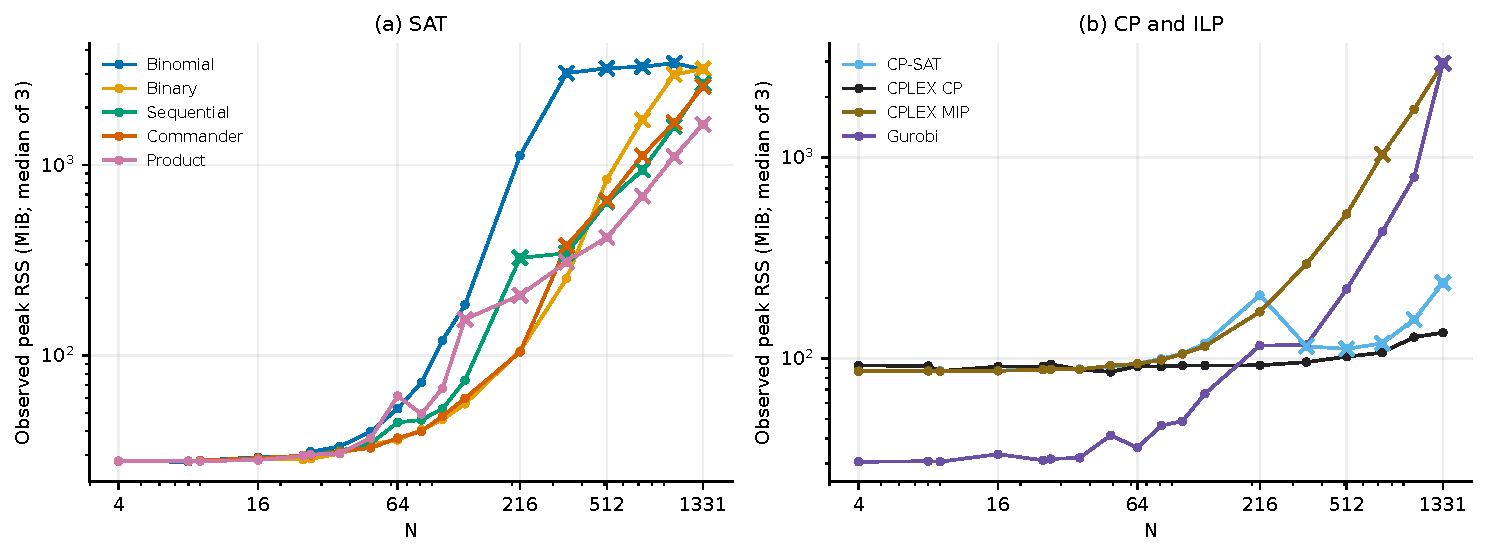
\includegraphics[width=\linewidth]{figures/memory.pdf}
\caption{Trung vị đỉnh RSS quan sát qua ba lượt, kể cả lượt chưa hoàn tất. Dấu x đánh dấu nhóm không hoàn tất đủ 3/3. Hai trục dùng thang log; các điểm bị ngắt không biểu diễn lượng RAM cần để giải thành công.}
\label{fig:memory}
\end{figure}
Tại $N=216$, Binomial dùng RSS đỉnh trung vị khoảng 1120.7 MiB; Binary 105.4 MiB và Commander 104.2 MiB. Ở đây CNF lớn của Binomial đi cùng chi phí nạp và bộ nhớ cao. Tuy nhiên, tại $N=64$, Product có ít clause nhất nhưng RSS 61.2 MiB, cao hơn Binary 36.0 MiB: bộ nhớ còn chứa trạng thái tìm kiếm và clause học, không chỉ công thức đầu vào.

Tại $N=1331$, CPLEX CP hoàn tất với RSS trung vị khoảng 134.3 MiB; Product bị timeout với RSS quan sát trung vị 1634.2 MiB. Hai con số không phải so sánh bộ nhớ để cùng hoàn thành bài toán. Giá trị RSS lớn nhất trong cả 486 lượt là 4631.2 MiB, vẫn dưới ngưỡng cấu hình 6144 MiB; bộ dữ liệu không có MEM\_LIMIT. Điều này chỉ mô tả những gì đã quan sát trước khi các lượt dừng, không chứng minh mọi phương pháp sẽ đủ RAM nếu bỏ giới hạn thời gian.

\subsection{Các lượt bị giới hạn và trường hợp thành công một phần}
\begin{table}[pos=H]
\centering
\footnotesize
\caption{Ba lượt Product đệ quy tại N=125.}
\label{tab:partial_product}
\setlength{\tabcolsep}{4pt}
\begin{tabular}{@{}lrrrrrr@{}}
\toprule
Lượt & Trạng thái & Build (s) & Load (s) & Solve (s) & Total (s) & RSS (MiB) \\
\midrule
1 & SAT & 0.0864 & 0.1827 & 91.748 & 92.942 & 185.1 \\
2 & TIMEOUT & 0.0742 & 0.1598 & -- & 100.027 & 138.4 \\
3 & TIMEOUT & 0.0754 & 0.1525 & -- & 100.019 & 154.8 \\
\bottomrule
\end{tabular}
\par\smallskip\begin{minipage}{\linewidth}\footnotesize Cả ba lượt đã nạp đủ 161.882 clause. Build/load của lượt TIMEOUT là số ghi nhận gần nhất; solve chưa hoàn tất nên không dùng giá trị 0 trong log. Không công bố trung vị hoàn tất của cả cấu hình từ một lượt SAT.\end{minipage}
\end{table}

Product tại $N=125$ là trường hợp duy nhất chỉ thành công một phần: lượt 1 có total 92.942 giây, lượt 2 và 3 timeout xấp xỉ 100 giây. Cả ba đã nạp đủ 161\,882 clause. Vì hai thời gian hoàn tất chưa quan sát được, 92.942 giây không được dùng làm trung vị thời gian hoàn tất của cấu hình. Bảng chính ghi 1S+2TO và bảng chi tiết giữ từng lượt.

\begin{table}[pos=H]
\centering
\small
\caption{Tiến độ nạp CNF trong các lượt SAT bị TIMEOUT.}
\label{tab:timeout_progress}
\setlength{\tabcolsep}{4pt}
\begin{tabular}{@{}lrrr@{}}
\toprule
Encoding & Số TO & Đã báo nạp đủ & Chưa báo nạp đủ \\
\midrule
Binomial & 15 & 3 & 12 \\
Binary & 9 & 6 & 3 \\
Sequential & 18 & 18 & 0 \\
Commander & 15 & 15 & 0 \\
Product & 20 & 20 & 0 \\
\bottomrule
\end{tabular}
\par\smallskip\begin{minipage}{\linewidth}\footnotesize Tiến độ là thông báo gần nhất. Đã nạp đủ không có nghĩa đã giải xong; nhãn phase có thể cũ. Không lấy solve\_s=0 của lượt bị ngắt làm thời gian tìm kiếm.\end{minipage}
\end{table}

Trong 77 lượt TIMEOUT của các phương pháp SAT, 62 lượt đã báo nạp đủ CNF và 15 lượt chưa báo nạp đủ. Các lượt Sequential, Commander và Product bị timeout đều thuộc nhóm đã nạp đủ. Vì thông báo pha có thể chậm hơn tiến trình thực, báo cáo dùng bộ đếm clause để phân biệt tiến độ, không chỉ dựa vào nhãn \texttt{phase}.

\begin{table}[pos=H]
\centering
\footnotesize
\caption{Kích thước đầy đủ và tiến độ nạp tại N=1331.}
\label{tab:progress_1331}
\setlength{\tabcolsep}{4pt}
\begin{tabular}{@{}lrrrr@{}}
\toprule
Encoding & Clause đầy đủ & Nạp: nhỏ nhất & Nạp: lớn nhất & Trạng thái \\
\midrule
Binomial & 3\,926\,372\,802 & 71\,680\,000 & 80\,928\,768 & 3TO \\
Binary & 75\,151\,050 & 65\,363\,968 & 65\,978\,368 & 3TO \\
Sequential & 21\,229\,450 & 21\,229\,450 & 21\,229\,450 & 3TO \\
Commander & 24\,787\,642 & 24\,787\,642 & 24\,787\,642 & 3TO \\
Product & 15\,533\,774 & 15\,533\,774 & 15\,533\,774 & 3TO \\
\bottomrule
\end{tabular}
\par\smallskip\begin{minipage}{\linewidth}\footnotesize Các giá trị nạp là bản cập nhật đã nhận trước khi ngắt. Không phải kích thước CNF rút gọn và không bao gồm clause học.\end{minipage}
\end{table}

Tại $N=1331$, Sequential, Commander và Product đều nạp đủ CNF nhưng không trả nghiệm được chấp nhận trước khi lượt bị dừng. Binomial và Binary chưa báo nạp đủ. Do đó không thể diễn giải tất cả TIMEOUT như việc solver đã được dành riêng đủ 100 giây để tìm kiếm. Tăng RAM đơn thuần cũng không trực tiếp giải quyết các trường hợp chạm thời gian khi RSS vẫn dưới ngưỡng.

\subsection{Đối chiếu tài liệu tham khảo và giới hạn của kết luận}
Bảng thời gian SAT được trình bày theo hàng $N$ và cột encoding, tương ứng cách tổ chức Bảng 4.2 trong tài liệu của Trần Ngọc Bách \citep{bach2024}. Tuy nhiên tài liệu đó dùng CPU i7-1165G7 và cài đặt khác; ở đây còn tách work với total và dùng ba lần lặp. Do đó không lấy tỷ số thời gian giữa hai báo cáo để kết luận encoder hiện tại nhanh hoặc chậm hơn do một thay đổi duy nhất. Tương tự, bộ dữ liệu này không phải phép so sánh có kiểm soát giữa bản một tầng và bản đệ quy.

Có bốn giới hạn cần giữ khi diễn giải. Thứ nhất, chỉ có một máy, một SAT backend và 18 bàn cờ trống; kết quả không đại diện cho N-Queens có hậu cố định hoặc các bài toán lực lượng khác. Thứ hai, ba lần lặp cùng cấu hình mô tả biến động thời gian nhưng không đủ suy diễn thống kê mạnh về mọi seed hay mọi môi trường. Thứ ba, giới hạn toàn lượt làm chi phí khởi động, dựng và nạp mô hình ảnh hưởng mức độ hoàn tất. Thứ tư, RSS lấy mẫu và số đếm mô hình có ý nghĩa khác nhau giữa các họ bộ giải.

Manifest có hash mã nguồn nhưng gói kết quả không thay thế snapshot nguồn tương ứng hoặc commit Git. Phiên bản CP Optimizer engine, tên thương mại CPU và trạng thái nguồn điện cần được bổ sung nếu muốn tái lập sát môi trường gốc. Các kết luận trong báo cáo giới hạn ở cài đặt được mô tả và những số đo đã cung cấp.


\subsection{Tái tạo số liệu và truy vết biểu đồ}
\label{sec:reproducibility}
Quy trình hậu xử lý sử dụng một nguồn thống kê chung cho bảng và hình. Trước khi tổng hợp, chương trình đối chiếu từng trường CSV với bản ghi JSONL theo run ID, kiểm tra đủ lưới 486 lượt và kiểm tra nghiệm. Sau đó các lượt được nhóm theo cặp $(N,\text{phương pháp})$; work được cộng trong từng lượt trước khi tính trung vị. Nhóm chưa hoàn tất đủ ba lần không được đưa vào đường thời gian như một điểm hoàn tất; trạng thái của nó được giữ trong bảng và Hình~\ref{fig:status}.

Số liệu dẫn xuất được lưu vào \texttt{summary\_report.csv}. Khi vẽ, chương trình đồng thời xuất chính các điểm đã sử dụng sang CSV tương ứng từng hình. Nhờ đó, một điểm có thể được kiểm tra ngược qua ba mức: CSV của hình, dòng tổng hợp và ba bản ghi gốc. Chẳng hạn Product tại $N=125$ giữ trạng thái 1S+2TO và không có trung vị hoàn tất trong đường thời gian; lượt thành công vẫn được trình bày riêng ở bảng phân tích thành công một phần. Với hình phân rã pha, CSV giữ run ID của lượt có total trung vị, bảo đảm các thành phần của một cột thuộc cùng một lượt thật.

Sau khi tách mã hậu xử lý thành các module, toàn bộ 24 bảng thực nghiệm, bốn CSV tổng hợp và kết quả audit đã được đối chiếu với bản dựng trước và giữ nguyên số liệu. Sáu kiểm thử kiểm tra các rủi ro tổng hợp: cộng pha trước trung vị; giữ nhóm thành công một phần; phát hiện run ID trùng và số đo CSV/JSONL không khớp; đối chiếu điểm hình với thống kê; và kiểm tra tổng các pha của đúng một lượt. Đây là kiểm chứng phần hậu xử lý, không phải kiểm thử thêm các solver. Chi tiết lệnh chạy và vai trò từng hình ở Phụ lục~\ref{app:reproduce}.

\FloatBarrier
\section{Conclusion}
\label{sec:conclusion}
Báo cáo xây dựng mô hình SAT N-Queens bằng $N^2$ biến ô cờ, ALO/AMO trên hàng và cột, cùng AMO trên hai họ đường chéo. Năm mã hóa sử dụng cùng tập bố trí hậu hợp lệ nhưng khác cách tổ chức biến phụ và mệnh đề. Commander nhóm tối đa ba biến và Product tọa độ được áp dụng đệ quy; Sequential dùng chuỗi Sinz với ngưỡng Pairwise cho nhóm không quá ba biến. Những lựa chọn này được nêu bằng công thức, ví dụ, lập luận tính đúng và công thức đếm, thay vì chỉ dựa vào tên của họ encoding.

Đợt thực nghiệm gồm 486 lượt trên 18 kích thước, tạo 385 nghiệm đã kiểm tra hợp lệ, 99 TIMEOUT và hai UNKNOWN. Không có lượt bị bỏ qua theo kích thước CNF. Theo tiêu chí hoàn tất đủ ba lần lặp, CPLEX CP đạt 18/18 kích thước, Gurobi 17/18, CPLEX MIP 16/18 và Binary 15/18. Binary có mức độ hoàn tất tốt nhất trong nhóm SAT hiện tại; Product hoàn tất 11/18 và thêm một lượt thành công tại $N=125$.

Các kết quả trả lời những câu hỏi nghiên cứu theo ba hướng. Thứ nhất, số clause nhỏ hơn không bảo đảm tìm nghiệm nhanh hơn: Product tại $N=64$ có ít clause nhất nhưng lượng xung đột, lan truyền và thời gian solve lớn. Thứ hai, chi phí sinh/nạp có thể chi phối ở CNF lớn, trong khi khởi động/thiết lập chi phối total ở $N$ nhỏ; vì vậy cần báo cáo đồng thời work và total. Thứ ba, timeout phải được đọc cùng tiến độ: tại $N=1331$, có mã hóa đã nạp đủ CNF và có mã hóa chưa nạp đủ trước khi bị dừng.

CPLEX CP cho kết quả tốt nhất về mức độ hoàn tất trong tập này, nhưng thực nghiệm đồng thời thay cả cách biểu diễn và backend. Kết luận chỉ áp dụng cho các bàn cờ trống, cấu hình và máy đã quan sát; không suy rộng thành thứ hạng chung giữa SAT, CP và ILP. Hướng phát triển phù hợp là thử thêm backend SAT, tăng số lần lặp có kiểm soát, đo riêng chế độ worker đã khởi động, và thiết kế phép đối chiếu từng thay đổi mã hóa dưới cùng điều kiện. Những mở rộng đó cần dữ liệu mới trước khi bổ sung kết luận về hiệu năng.

\section*{Data Availability}
Kho mã nguồn và kết quả: \RepositoryURL. Revision của bộ tái tạo: \RepositoryRevision.

Bộ dữ liệu sử dụng có định danh \texttt{20261015T101136Z\_afe2720f}. Bốn đầu vào gồm \texttt{experiment\_results.csv}, \texttt{results.jsonl}, \texttt{manifest.json} và \texttt{summary.csv}, dự kiến công bố tại \path{results/experiment_02/} trong repository. Gói báo cáo giữ bản sao nguyên nội dung tại \texttt{data/}; riêng summary được đổi tên thành \texttt{summary\_runner.csv} để phân biệt với số liệu dẫn xuất.

Mã hậu xử lý được tách trong \texttt{analysis/}: đọc/kiểm tra/thống kê tại \texttt{data\_processing.py}, xuất bảng tại \texttt{tables.py} và vẽ hình tại \texttt{plots.py}. Từ gốc repository, chạy \texttt{python -m analysis} với đầu vào \path{results/experiment_02} và đầu ra \texttt{report}. Lệnh đầy đủ và cách kiểm tra từng điểm được nêu tại Phụ lục~\ref{app:reproduce} và \texttt{HUONG\_DAN\_TAI\_TAO.md}. Hai mươi bốn bảng thực nghiệm và tám hình được tạo từ dữ liệu, không nhập số thủ công. Các bảng ký hiệu, công thức, môi trường và quy trình là phần mô tả trong LaTeX.

Mỗi hình có bản PDF, PNG và CSV điểm dữ liệu tại \path{report/data/figure_points/}. \texttt{data\_audit.json} lưu kiểm tra và SHA-256 đầu vào. Gói LaTeX độc lập đóng kèm cùng module \texttt{analysis/}; \texttt{build\_report.py} chỉ là lệnh gọi tiện dụng từ dữ liệu đã đóng gói. \texttt{README\_VI.md} hướng dẫn biên dịch XeLaTeX; \texttt{metadata.tex} chứa thông tin tác giả và repository cần điền.

Khi công bố, cần giữ snapshot hoặc commit triển khai solver đúng đợt thực nghiệm, ngoài mã hậu xử lý. \texttt{code\_hash} trong manifest là fingerprint của runner, không tự động là Git commit hash. Bộ tái tạo báo cáo không thay thế mã solver gốc. URL và revision đang để trống có đánh dấu; chưa thể coi yêu cầu liên kết repository là hoàn tất cho tới khi tác giả công bố và điền các trường này.

\section*{Ghi nhận hỗ trợ biên soạn}
ChatGPT hỗ trợ hệ thống hóa mô hình, tổng hợp dữ liệu và biên soạn LaTeX. Các số đo thực nghiệm do người thực hiện cung cấp; người thực hiện chịu trách nhiệm kiểm tra nội dung, đối chiếu với mã nguồn được nộp và hoàn thiện thông tin tái lập.

\FloatBarrier
\appendix
\section{Thời gian thành phần đầy đủ}
\label{app:phases}
Các bảng sau tách build/load/solve để đọc cùng work và total trong phần chính. Đơn vị là giây. Các giá trị rất nhỏ được giữ thêm chữ số để không bị hiển thị thành 0; điều này không hàm ý phép đo có độ chính xác tuyệt đối tới chữ số cuối.
\begin{table}[pos=H]
\centering
\small
\caption{Thời gian sinh CNF SAT (giây).}
\label{tab:sat_build}
\setlength{\tabcolsep}{4pt}
\begin{tabular}{@{}lrrrrr@{}}
\toprule
$N$ & Binomial & Binary & Sequential & Commander & Product \\
\midrule
4 & 0.000101 & 0.000145 & 0.000145 & 0.000219 & 0.000120 \\
8 & 0.000337 & 0.000425 & 0.000333 & 0.000560 & 0.000584 \\
9 & 0.000436 & 0.000571 & 0.000449 & 0.000743 & 0.000670 \\
16 & 0.004802 & 0.003365 & 0.002613 & 0.004080 & 0.003813 \\
25 & 0.009329 & 0.006029 & 0.004446 & 0.007701 & 0.006155 \\
27 & 0.0113 & 0.006435 & 0.004808 & 0.009049 & 0.007402 \\
36 & 0.0268 & 0.0121 & 0.006959 & 0.0133 & 0.0105 \\
49 & 0.0617 & 0.0252 & 0.0125 & 0.0232 & 0.0188 \\
64 & 0.1360 & 0.0372 & 0.0197 & 0.0388 & 0.0279 \\
81 & 0.2839 & 0.0639 & 0.0270 & 0.0570 & 0.0376 \\
100 & 0.5188 & 0.0995 & 0.0432 & 0.0918 & 0.0523 \\
125 & 1.121 & 0.1577 & 0.0598 & 0.1373 & 1S+2TO \\
216 & 5.943 & 0.5317 & TO & 0.3939 & TO \\
343 & TO & 1.532 & TO & TO & TO \\
512 & TO & 3.562 & TO & TO & TO \\
729 & TO & TO & TO & TO & TO \\
1000 & TO & TO & TO & TO & TO \\
1331 & TO & TO & TO & TO & TO \\
\bottomrule
\end{tabular}
\par\smallskip\begin{minipage}{\linewidth}\footnotesize Giá trị số: trung vị của ba lượt SAT có nghiệm hợp lệ. TO: ba TIMEOUT; 2TO+1U: hai TIMEOUT và một UNKNOWN; 1S+2TO: một SAT và hai TIMEOUT. Không thay lượt chưa hoàn tất bằng 0 hoặc 100 giây.\end{minipage}
\end{table}

\begin{table}[pos=H]
\centering
\small
\caption{Thời gian nạp CNF SAT (giây).}
\label{tab:sat_load}
\setlength{\tabcolsep}{4pt}
\begin{tabular}{@{}lrrrrr@{}}
\toprule
$N$ & Binomial & Binary & Sequential & Commander & Product \\
\midrule
4 & 0.000136 & 0.000187 & 0.000175 & 0.000203 & 0.000136 \\
8 & 0.000739 & 0.001215 & 0.000655 & 0.000703 & 0.000750 \\
9 & 0.000943 & 0.001127 & 0.000841 & 0.000904 & 0.001134 \\
16 & 0.008330 & 0.003618 & 0.002731 & 0.003581 & 0.002762 \\
25 & 0.0191 & 0.0110 & 0.007011 & 0.008278 & 0.008171 \\
27 & 0.0243 & 0.0128 & 0.007763 & 0.0106 & 0.009367 \\
36 & 0.0590 & 0.0246 & 0.0140 & 0.0179 & 0.0155 \\
49 & 0.1459 & 0.0474 & 0.0274 & 0.0339 & 0.0337 \\
64 & 0.3415 & 0.0863 & 0.0448 & 0.0556 & 0.0431 \\
81 & 0.6932 & 0.1495 & 0.0762 & 0.0893 & 0.0701 \\
100 & 1.315 & 0.2409 & 0.1190 & 0.1438 & 0.1045 \\
125 & 2.732 & 0.3835 & 0.1767 & 0.2278 & 1S+2TO \\
216 & 15.416 & 1.298 & TO & 0.7232 & TO \\
343 & TO & 4.263 & TO & TO & TO \\
512 & TO & 9.401 & TO & TO & TO \\
729 & TO & TO & TO & TO & TO \\
1000 & TO & TO & TO & TO & TO \\
1331 & TO & TO & TO & TO & TO \\
\bottomrule
\end{tabular}
\par\smallskip\begin{minipage}{\linewidth}\footnotesize Giá trị số: trung vị của ba lượt SAT có nghiệm hợp lệ. TO: ba TIMEOUT; 2TO+1U: hai TIMEOUT và một UNKNOWN; 1S+2TO: một SAT và hai TIMEOUT. Không thay lượt chưa hoàn tất bằng 0 hoặc 100 giây.\end{minipage}
\end{table}

\begin{table}[pos=H]
\centering
\small
\caption{Thời gian quanh lời gọi giải SAT (giây).}
\label{tab:sat_solve}
\setlength{\tabcolsep}{4pt}
\begin{tabular}{@{}lrrrrr@{}}
\toprule
$N$ & Binomial & Binary & Sequential & Commander & Product \\
\midrule
4 & 0.000061 & 0.000085 & 0.000064 & 0.000079 & 0.000063 \\
8 & 0.000265 & 0.000334 & 0.000212 & 0.000641 & 0.000670 \\
9 & 0.000154 & 0.000459 & 0.000261 & 0.000557 & 0.000863 \\
16 & 0.0178 & 0.0111 & 0.0110 & 0.0702 & 0.007254 \\
25 & 0.005146 & 0.0139 & 0.0421 & 0.0209 & 0.0211 \\
27 & 0.0163 & 0.007481 & 0.0906 & 0.0446 & 0.0832 \\
36 & 0.008011 & 0.0567 & 0.1181 & 0.0870 & 0.0740 \\
49 & 0.006487 & 0.1920 & 0.5517 & 0.0614 & 0.7420 \\
64 & 0.0229 & 0.1026 & 3.839 & 0.2145 & 18.884 \\
81 & 0.1186 & 0.1314 & 2.839 & 0.2276 & 3.541 \\
100 & 0.0554 & 0.1014 & 4.554 & 1.158 & 17.169 \\
125 & 0.0874 & 0.1873 & 16.062 & 2.650 & 1S+2TO \\
216 & 1.237 & 0.4549 & TO & 2.818 & TO \\
343 & TO & 2.300 & TO & TO & TO \\
512 & TO & 66.373 & TO & TO & TO \\
729 & TO & TO & TO & TO & TO \\
1000 & TO & TO & TO & TO & TO \\
1331 & TO & TO & TO & TO & TO \\
\bottomrule
\end{tabular}
\par\smallskip\begin{minipage}{\linewidth}\footnotesize Giá trị số: trung vị của ba lượt SAT có nghiệm hợp lệ. TO: ba TIMEOUT; 2TO+1U: hai TIMEOUT và một UNKNOWN; 1S+2TO: một SAT và hai TIMEOUT. Không thay lượt chưa hoàn tất bằng 0 hoặc 100 giây.\end{minipage}
\end{table}

\begin{table}[pos=H]
\centering
\small
\caption{Thời gian xây mô hình CP/ILP (giây).}
\label{tab:native_build}
\setlength{\tabcolsep}{4pt}
\begin{tabular}{@{}lrrrr@{}}
\toprule
$N$ & CP-SAT & CPLEX CP & CPLEX MIP & Gurobi \\
\midrule
4 & 0.001613 & 0.001550 & 0.003312 & 0.002651 \\
8 & 0.001404 & 0.001431 & 0.004678 & 0.003296 \\
9 & 0.002194 & 0.001688 & 0.004702 & 0.003258 \\
16 & 0.001679 & 0.001360 & 0.008655 & 0.007264 \\
25 & 0.001928 & 0.001458 & 0.0151 & 0.0136 \\
27 & 0.002086 & 0.001694 & 0.0155 & 0.0140 \\
36 & 0.002265 & 0.001576 & 0.0240 & 0.0241 \\
49 & 0.002977 & 0.001628 & 0.0376 & 0.0424 \\
64 & 0.003134 & 0.001833 & 0.0629 & 0.0662 \\
81 & 0.003520 & 0.002371 & 0.0812 & 0.1047 \\
100 & 0.0114 & 0.002150 & 0.1203 & 0.1558 \\
125 & 0.004471 & 0.002480 & 0.2021 & 0.2309 \\
216 & 0.006869 & 0.003330 & 0.6064 & 0.7344 \\
343 & 2TO+1U & 0.004576 & 1.529 & 1.877 \\
512 & TO & 0.006161 & 3.817 & 4.462 \\
729 & 2TO+1U & 0.008833 & TO & 10.068 \\
1000 & TO & 0.0124 & 16.685 & 20.251 \\
1331 & TO & 0.0168 & TO & TO \\
\bottomrule
\end{tabular}
\par\smallskip\begin{minipage}{\linewidth}\footnotesize Giá trị số: trung vị của ba lượt SAT có nghiệm hợp lệ. TO: ba TIMEOUT; 2TO+1U: hai TIMEOUT và một UNKNOWN; 1S+2TO: một SAT và hai TIMEOUT. Không thay lượt chưa hoàn tất bằng 0 hoặc 100 giây.\end{minipage}
\end{table}

\begin{table}[pos=H]
\centering
\small
\caption{Thời gian quanh lời gọi giải CP/ILP (giây).}
\label{tab:native_solve}
\setlength{\tabcolsep}{4pt}
\begin{tabular}{@{}lrrrr@{}}
\toprule
$N$ & CP-SAT & CPLEX CP & CPLEX MIP & Gurobi \\
\midrule
4 & 0.0109 & 0.0678 & 0.008737 & 0.007854 \\
8 & 0.0203 & 0.0629 & 0.007844 & 0.006175 \\
9 & 0.0222 & 0.0604 & 0.008861 & 0.005898 \\
16 & 0.0442 & 0.0556 & 0.0130 & 0.0320 \\
25 & 0.0943 & 0.0641 & 0.0190 & 0.006594 \\
27 & 0.1091 & 0.0594 & 0.0197 & 0.006246 \\
36 & 0.2132 & 0.0605 & 0.0298 & 0.007075 \\
49 & 0.4231 & 0.0602 & 0.0457 & 0.1496 \\
64 & 0.7286 & 0.0696 & 0.0770 & 0.009394 \\
81 & 1.392 & 0.0714 & 0.1084 & 0.2311 \\
100 & 3.342 & 0.0706 & 0.1740 & 0.2749 \\
125 & 4.953 & 0.0707 & 0.2679 & 0.9562 \\
216 & 29.904 & 0.0830 & 1.150 & 1.936 \\
343 & 2TO+1U & 0.0994 & 3.436 & 0.0926 \\
512 & TO & 0.1766 & 7.089 & 0.2577 \\
729 & 2TO+1U & 0.2066 & TO & 0.6932 \\
1000 & TO & 0.4581 & 55.126 & 1.616 \\
1331 & TO & 0.5043 & TO & TO \\
\bottomrule
\end{tabular}
\par\smallskip\begin{minipage}{\linewidth}\footnotesize Giá trị số: trung vị của ba lượt SAT có nghiệm hợp lệ. TO: ba TIMEOUT; 2TO+1U: hai TIMEOUT và một UNKNOWN; 1S+2TO: một SAT và hai TIMEOUT. Không thay lượt chưa hoàn tất bằng 0 hoặc 100 giây.\end{minipage}
\end{table}

\FloatBarrier
\section{Độ phân tán và cách tính}
\label{app:dispersion}
\begin{table}[pos=H]
\centering
\footnotesize
\caption{Độ phân tán mô tả của $T_{work}$ tại một số kích thước.}
\label{tab:dispersion}
\setlength{\tabcolsep}{4pt}
\begin{tabular}{@{}lrrrr@{}}
\toprule
$N$ & Encoding & Trung vị (s) & IQR (s) & IQR/trung vị (\%) \\
\midrule
4 & Binomial & 0.000295 & 0.000004 & 1.4 \\
4 & Binary & 0.000424 & 0.000027 & 6.4 \\
4 & Sequential & 0.000388 & 0.000050 & 13.0 \\
4 & Commander & 0.000500 & 0.000127 & 25.5 \\
4 & Product & 0.000322 & 0.000005 & 1.6 \\
64 & Binomial & 0.5004 & 0.0153 & 3.1 \\
64 & Binary & 0.2273 & 0.009226 & 4.1 \\
64 & Sequential & 3.902 & 0.1286 & 3.3 \\
64 & Commander & 0.3088 & 0.0153 & 4.9 \\
64 & Product & 18.958 & 0.5619 & 3.0 \\
81 & Binomial & 1.091 & 0.0968 & 8.9 \\
81 & Binary & 0.3448 & 0.1239 & 35.9 \\
81 & Sequential & 2.945 & 0.1090 & 3.7 \\
81 & Commander & 0.3738 & 0.0145 & 3.9 \\
81 & Product & 3.648 & 0.3666 & 10.0 \\
216 & Binomial & 22.912 & 0.6474 & 2.8 \\
216 & Binary & 2.296 & 0.0679 & 3.0 \\
216 & Commander & 3.940 & 0.0383 & 1.0 \\
512 & Binary & 81.088 & 7.642 & 9.4 \\
\bottomrule
\end{tabular}
\par\smallskip\begin{minipage}{\linewidth}\footnotesize Q1/Q3 dùng nội suy inclusive trên ba lượt hoàn tất. IQR không phải khoảng tin cậy; không áp dụng bảng này cho nhóm Product N=125 chỉ có một lượt SAT.\end{minipage}
\end{table}

Với ba giá trị đã sắp $t_1\le t_2\le t_3$, trung vị là $t_2$. Nội suy inclusive cho $Q_1=(t_1+t_2)/2$, $Q_3=(t_2+t_3)/2$, nên IQR $=(t_3-t_1)/2$. Script tính trên work của từng lượt, không cộng trung vị riêng của các pha. File \texttt{data/summary\_report.csv} lưu toàn bộ trung vị, Q1/Q3 và trạng thái nhóm. Các cột có tên \texttt{median\_completed} chỉ mô tả các lượt thành công, không được dùng thay cho trung vị của nhóm đủ ba lượt trong bảng chính.

\section{Số literal và ý nghĩa của số đếm}
Binomial, Binary, Sequential và Product đang dùng chỉ có clause AMO hai literal, nên $\ell_E(k)=2c_E(k)$. Commander có điều kiện dừng $\ell_C(k)=2\binom k2$ khi $k\le3$. Với $k>3$:
\[
\ell_C(k)=2I(k)+3k+m+\ell_C(m),\qquad m=\lceil k/3\rceil.
\]
Ba hạng ở tầng hiện tại gồm $2I(k)$ literal nội nhóm, $2k$ literal từ đầu vào đến commander và $k+m$ literal của liên kết chiều ngược. Product cũng có thể được viết dưới dạng truy hồi $\ell_P(k)=4k+\ell_P(p)+\ell_P(q)$ khi $k>4$.

ALO đóng góp $N^2(1+d)$ literal, với $d$ là cờ ALO cột. Toàn bàn cờ có
\[
L_E(N)=N^2(1+d)+(2N+2)\ell_E(N)+4\sum_{k=2}^{N-1}\ell_E(k).
\]
Công thức đúng với các ngưỡng và clause cụ thể đã mô tả. Thay nhóm, ngưỡng dừng hoặc liên kết phải cập nhật công thức và kiểm tra lại với generator. Tổng biến được tính là biến chính cộng biến phụ đã cấp; ID lớn nhất chỉ bằng số biến khi cách cấp ID liên tục và các biến được tính đều xuất hiện.

\section{Đối chiếu yêu cầu và khả năng tái lập}
\begin{table}[pos=H]\centering\small
\caption{Các nội dung đáp ứng yêu cầu Bài tập lớn số 1.}
\begin{tabular}{@{}p{.40\linewidth}p{.53\linewidth}@{}}\toprule
Nội dung & Vị trí trong báo cáo\\\midrule
Giải N-Queens bằng SAT/PySAT & Mô hình CNF, năm encoder và quy trình Glucose3 tại Phần~\ref{sec:methodology}.\\
So sánh CPLEX CP, CPLEX MIP, Gurobi, CP-SAT & Mô hình CP/MIP tại Phần~\ref{sec:methodology}; thời gian, coverage và RAM tại Phần~\ref{sec:experiments}.\\
Thực nghiệm kích thước lớn & 18 kích thước đến 1331; mọi cấu hình đều được thử, không có SKIPPED.\\
Trình bày ALO/AMO & Định nghĩa tại Background; CNF, ví dụ, tính đúng, số đếm tại Methodology.\\
Hình thức bài báo khoa học & Lớp \texttt{cas-sc}; abstract, năm phần chính, Data Availability và tài liệu tham khảo.\\
Liên kết mã nguồn và kết quả & Mã tái tạo tại Phụ lục~\ref{app:reproduce}; URL repository và commit/tag còn cần tác giả điền.\\
\bottomrule\end{tabular}
\end{table}
Các thông tin chưa có trong đầu vào được để rõ để hoàn thiện trước khi nộp: mã sinh viên, lớp/mã học phần, trường/khoa, xác nhận thông tin giảng viên, URL repository và commit/tag mã nguồn. Để tái lập sát môi trường hơn, cần bổ sung tên thương mại CPU, phiên bản executable CP Optimizer và chế độ nguồn điện khi chạy. Không còn phần thực nghiệm đệ quy để trống: Commander và Product trong toàn bộ bảng hiện tại đã là đệ quy.

Tệp manifest lưu fingerprint mã nguồn và cấu hình; script tổng hợp lưu SHA-256 của từng tệp đầu vào trong \texttt{data\_audit.json}. Các dấu vân tay hỗ trợ phát hiện trộn dữ liệu hoặc thay đầu vào, nhưng không thay thế việc công bố mã nguồn. Script cố ý kiểm tra đúng đợt và đúng cấu hình hiện tại; nếu chạy một thí nghiệm khác, cần tạo báo cáo riêng và cập nhật mô tả, không chỉ thay CSV rồi giữ nguyên diễn giải.


\FloatBarrier
\section{Quy trình tái tạo bảng và biểu đồ}
\label{app:reproduce}
Phần hậu xử lý độc lập với các bộ giải. Nó chỉ đọc kết quả đã có và có thể chạy lại nhiều lần để sửa cách trình bày mà không chạy lại thực nghiệm. Tại gốc dự án, cài phụ thuộc trong \texttt{requirements-analysis.txt}, rồi chạy:
\begin{quote}\small\ttfamily
python -m analysis --input results/experiment\_02 --output report
\end{quote}
Đầu vào phải thuộc đợt và biến thể được phân tích; kiểm tra experiment ID/cấu hình giúp ngăn trộn kết quả một tầng với bản đệ quy. Để tái tạo từ bản sao trong gói, dùng \texttt{--input report/data}. Với gói LaTeX độc lập, lệnh \texttt{python build\_report.py} gọi cùng bộ xử lý trên \texttt{data/}.

\begin{table}[pos=H]\centering\small
\caption{Các bước từ dữ liệu gốc đến bảng và hình.}
\begin{tabular}{@{}p{.25\linewidth}p{.68\linewidth}@{}}\toprule
Thành phần & Vai trò và đầu ra\\\midrule
\path{analysis/__main__.py} & Đọc tham số, gọi kiểm tra, tổng hợp, xuất bảng và vẽ; không gọi solver.\\
\path{data_processing.py} & Đối chiếu bốn đầu vào, nhóm theo $N$--phương pháp, tính trung vị/IQR, số đếm và mức độ hoàn tất.\\
\path{tables.py} & Tạo 24 tệp bảng thực nghiệm tại \texttt{report/tables/}; giữ trạng thái thay cho số chưa biết.\\
\path{plots.py} & Tạo tám hình PDF/PNG cùng CSV điểm hình tại \path{report/data/figure_points/}.\\
\path{tests/test_report_analysis.py} & Sáu kiểm thử cho tính đúng của hậu xử lý và khả năng truy vết.\\
\path{report/main.tex} & Ghép văn bản, bảng và hình; biên dịch bằng XeLaTeX.\\
\bottomrule\end{tabular}
\end{table}

\begin{table}[pos=H]\centering\small
\caption{Câu hỏi và quy tắc dữ liệu của tám hình (tên tệp không kèm phần mở rộng).}
\begin{tabular}{@{}p{.25\linewidth}p{.68\linewidth}@{}}\toprule
Tên hình & Mục đích và cách đọc\\\midrule
\texttt{formula\_sizes} & CNF tăng ra sao theo $N$? Vẽ tổng biến và clause đầy đủ theo công thức, kể cả nhóm timeout; không phải tiến độ đã sinh.\\
\texttt{sat\_runtime} & Encoding SAT nào nhanh hơn? Vẽ median work và total; chỉ nhóm hoàn tất 3/3.\\
\texttt{native\_runtime} & SAT so với CP/ILP thế nào? Cùng quy tắc thời gian; so sánh đồng thời mô hình và backend.\\
\texttt{memory} & RSS quan sát tăng thế nào? Median đỉnh RSS cả ba lượt; dấu $\times$ chỉ nhóm chưa hoàn tất 3/3.\\
\texttt{status\_matrix} & Phương pháp giải được những $N$ nào? Mỗi ô giữ đủ trạng thái của ba lượt, gồm UNKNOWN và thành công một phần.\\
\texttt{cactus} & Bao nhiêu kích thước hoàn tất dưới một ngưỡng median total? Trục ngang là thời gian, trục dọc đếm kích thước hoàn tất 3/3.\\
\texttt{sat\_iqr} & Ba lượt dao động ra sao? Median và khoảng Q1--Q3 của work ở nhóm đủ 3/3; không phải khoảng tin cậy.\\
\texttt{phase\_breakdown} & Total lớn do pha nào? Chồng pha của một lượt thật có total trung vị tại $N=4,216$.\\
\bottomrule\end{tabular}
\end{table}

Để kiểm tra một điểm, chạy \texttt{python -m analysis} với \texttt{--input results/experiment\_02 --inspect 64 Binary}. Chương trình in ba lượt và thống kê của nhóm mà không ghi tệp. Đối chiếu trường \texttt{median\_work\_s} với \texttt{summary\_report.csv}, rồi đối chiếu hàng $N=64$, phương pháp Binary, chỉ số median work trong \texttt{figure\_points/sat\_runtime.csv}. Để vẽ riêng hình thời gian SAT, thêm \texttt{--figure sat\_runtime} vào lệnh tạo báo cáo. Bỏ tùy chọn này để tạo toàn bộ bảng và hình.

Các trục log giúp biểu diễn đồng thời nhiều bậc độ lớn: khoảng cách bằng nhau ứng với tỷ số bằng nhau, không phải chênh lệch tuyệt đối bằng nhau. Giá trị thiếu không được thay bằng 0 để vẽ. Đường nối các điểm chỉ hỗ trợ quan sát các kích thước đã thử, không khẳng định thời gian cho các $N$ chưa thực nghiệm. Hình cactus không giữ trục $N$; mỗi bước tăng là một kích thước hoàn tất có median total đạt ngưỡng tương ứng, không phải thời gian tích lũy chạy tất cả bài toán.

Với hình phân rã pha, trường \texttt{coordination} là phần dư giữa total và tổng các pha đã ghi. Đây là giá trị suy ra, không phải số đo trực tiếp một pha mới. Native không có pha load riêng; phần load bằng 0 khi chồng cột chỉ là cách biểu diễn ``không áp dụng''. CSV lưu cờ \texttt{measured}, run ID và số lần lặp để phân biệt. Bảng thành phần có thể trình bày trung vị từng cột, nhưng hình chồng bắt buộc dùng các pha của cùng một lượt để tổng khớp total.

Để kiểm tra mã hậu xử lý, chạy \texttt{python -m unittest discover} với \texttt{-s tests -p test\_report\_analysis.py -v} từ gốc repository sau khi đã tạo đủ hình. Các kiểm thử không gọi lại solver. Môi trường tạo báo cáo được ghi trong \texttt{report\_build\_environment.json}, tách khỏi môi trường chạy solver trong manifest. Khác phiên bản Matplotlib có thể làm thay đổi nhỏ bố cục hình, trong khi các giá trị CSV cần được giữ nguyên.

Repository cần chứa đồng thời mã solver đúng đợt, bốn đầu vào, module \texttt{analysis/}, hướng dẫn, kiểm thử và nguồn báo cáo. Tệp khóa chạy, môi trường ảo và giấy phép thương mại không phải thành phần dữ liệu công bố. Hướng dẫn PowerShell từng bước, cách sửa hình và danh sách tệp cần commit nằm trong \texttt{HUONG\_DAN\_TAI\_TAO.md}. Không có thao tác push GitHub tự động trong bộ mã phân tích.

\FloatBarrier
\begin{thebibliography}{10}
\bibitem{assignment} Học phần Các vấn đề hiện đại KHMT. \emph{Yêu cầu Bài tập lớn số 1}, học kỳ I năm học 2026--2027. Tài liệu đề bài được cung cấp.
\bibitem{courseTemplate} Phạm Quang Minh, Đào Xuân Nghĩa, Tô Văn Khanh. \emph{Exact SAT Solving for the Two-Dimensional Bandwidth Minimization Problem}. Bản thảo dùng làm mẫu báo cáo học phần, 2026.
\bibitem{bach2024} Trần Ngọc Bách. \emph{An optimized SAT approach solving N-Queens problem}. Technology Project Report, University of Engineering and Technology, VNU, 2024.
\bibitem{amoSlides} Tô Văn Khanh. \emph{At Most One -- AMO, At Least One -- ALO Encoding}. Slide Module 3, trang 3--16; tài liệu học phần được cung cấp.
\bibitem{sinz2005} Carsten Sinz. Towards an Optimal CNF Encoding of Boolean Cardinality Constraints. \emph{Principles and Practice of Constraint Programming -- CP 2005}, 827--831. \url{https://www.carstensinz.de/papers/CP-2005.pdf}.
\bibitem{klieber2007} Will Klieber, Gihwon Kwon. \emph{Efficient CNF Encoding for Selecting 1 from N Objects}. 2007. \url{https://www.cs.cmu.edu/~wklieber/papers/2007_efficient-cnf-encoding-for-selecting-1.pdf}.
\end{thebibliography}

\end{document}
